% This is paper draft
% edited by Haoruo Peng
% Date: 2013.6.14
\documentclass[10pt, conference, compsocconf]{IEEEtran}
\usepackage{amsmath, amssymb}
\usepackage{color}
\usepackage{graphicx}
\usepackage{bbding}
\usepackage{epstopdf}

\newcommand{\bw}{\mathbf{w}}
\newcommand{\bwep}{\mathbf{w}^{\varepsilon}}
\newcommand{\bwfly}{\tilde{\mathbf{w}}}
\newcommand{\bwavg}{\mathbf{wavg}}
\newcommand{\bu}{\mathbf{u}}
\newcommand{\buprev}{\mathbf{uprev}}
\newcommand{\bp}{\mathbf{p}}
\newcommand{\bq}{\mathbf{q}}
\newcommand{\bxi}{\mathbf{\xi}}
\newcommand{\dotwxb}{{\mathbf{w}}^{\mathbf{T}}\mathbf{x}_{i}+b}
\newcommand{\sumt}{\sum_{t=1}^{T} }
\newcommand{\lc}{\left(}
\newcommand{\rc}{\right)}
\newcommand{\li}{\lc i\rc}
\newcommand{\lj}{\lc j\rc}
\newcommand{\tspace}{\hspace*{2em}}
\newcommand{\tspaces}{\hspace*{1.5em}}
\newcommand{\comment}{\textcolor{red}}
\newcommand{\ti}[1]{\tilde{#1}}
\newcommand{\indep}{{\;\bot\!\!\!\!\!\!\bot\;}}

\def\A{{\bf A}}
\def\a{{\bf a}}
\def\B{{\bf B}}
\def\C{{\bf C}}
\def\c{{\bf c}}
\def\D{{\bf D}}
\def\d{{\bf d}}
\def\E{{\bf E}}
\def\e{{\bf e}}
\def\f{{\bf f}}
\def\K{{\bf K}}
\def\H{{\bf H}}
\def\G{{\bf G}}
\def\I{{\bf I}}
\def\R{{\bf R}}
\def\X{{\bf X}}
\def\Y{{\bf Y}}
\def\Q{{\bf Q}}
\def\s{{\bf s}}
\def\S{{\bf S}}
\def\x{{\bf x}}
\def\y{{\bf y}}
\def\z{{\bf z}}
\def\Z{{\bf Z}}
\def\M{{\bf M}}
\def\m{{\bf m}}
\def\n{{\bf n}}
\def\U{{\bf U}}
\def\u{{\bf u}}
\def\V{{\bf V}}
\def\v{{\bf v}}
\def\W{{\bf W}}
\def\w{{\bf w}}
\def\0{{\bf 0}}
\def\1{{\bf 1}}

\def\AM{{\mathcal A}}
\def\FM{{\mathcal F}}
\def\TM{{\mathcal T}}
\def\UM{{\mathcal U}}
\def\XM{{\mathcal X}}
\def\YM{{\mathcal Y}}
\def\NM{{\mathcal N}}
\def\OM{{\mathcal O}}
\def\IM{{\mathcal I}}
\def\GM{{\mathcal G}}
\def\RB{{\mathbb R}}

\def\tx{\tilde{\bf x}}
\def\ty{\tilde{\bf y}}
\def\tz{\tilde{\bf z}}
\def\hd{\hat{d}}
\def\HD{\hat{\bf D}}
\def\hx{\hat{\bf x}}

\def\alp{\mbox{\boldmath$\alpha$\unboldmath}}
\def\bet{\mbox{\boldmath$\beta$\unboldmath}}
\def\epsi{\mbox{\boldmath$\epsilon$\unboldmath}}
\def\etab{\mbox{\boldmath$\eta$\unboldmath}}
\def\ph{\mbox{\boldmath$\phi$\unboldmath}}
\def\pii{\mbox{\boldmath$\pi$\unboldmath}}
\def\Ph{\mbox{\boldmath$\Phi$\unboldmath}}
\def\Ps{\mbox{\boldmath$\Psi$\unboldmath}}
\def\tha{\mbox{\boldmath$\theta$\unboldmath}}
\def\Tha{\mbox{\boldmath$\Theta$\unboldmath}}
\def\muu{\mbox{\boldmath$\mu$\unboldmath}}
\def\Si{\mbox{\boldmath$\Sigma$\unboldmath}}
\def\Gam{\mbox{\boldmath$\Gamma$\unboldmath}}
\def\Lam{\mbox{\boldmath$\Lambda$\unboldmath}}
\def\De{\mbox{\boldmath$\Delta$\unboldmath}}
\def\vps{\mbox{\boldmath$\varepsilon$\unboldmath}}

\def\Ncal{\mathcal{N}}
\def\argmax{\mathop{\rm argmax}}
\def\argmin{\mathop{\rm argmin}}

\def\sgn{\mathrm{sgn}}
\def\tr{\mathrm{tr}}
\def\rk{\mathrm{rank}}
\def\diag{\mathsf{diag}}
\def\vect{\mathsf{vec}}
\def\etal{{\em et al.\/}\,}

%\newtheorem{theorem}{Theorem}
%\newtheorem{lemma}{Lemma}
%\newtheorem{definition}{Definition}
%\newtheorem{proposition}{Proposition}
%\newtheorem{corollary}{Corollary}
%\newtheorem{example}{Example}

\begin{document}
%\mainmatter  % start of an individual contribution

% first the title is needed
\title{Learning for Penalized Logistic Regression Model in Parallel}

% a short form should be given in case it is too long for the running head
%\titlerunning{Learning for Penalized Logistic Regression Model in Parallel}

\author{\IEEEauthorblockN{Authors Name/s per 1st Affiliation (Author)}
\IEEEauthorblockA{line 1 (of Affiliation): dept. name of organization\\
line 2: name of organization, acronyms acceptable\\
line 3: City, Country\\
line 4: Email: name@xyz.com}
\and
\IEEEauthorblockN{Authors Name/s per 2nd Affiliation (Author)}
\IEEEauthorblockA{line 1 (of Affiliation): dept. name of organization\\
line 2: name of organization, acronyms acceptable\\
line 3: City, Country\\
line 4: Email: name@xyz.com}
}
%
%\author{Haoruo Peng\inst{1, 2}  \and Ding Liang\inst{1} \and Cyrus Choi\inst{1} \and Edward Y. Chang\inst{1} \and Yin Zhao\inst{2}}
%
%\authorrunning{Haoruo Peng \and Ding Liang \and Cyrus Choi \and Edward Y. Chang \and Yin Zhao}
% (feature abused for this document to repeat the title also on left hand pages)

%\institute %
%{
%\inst{}
%HTC Research, Beijing, China 100084 \\
%\and
%\inst{}
%Department of Computer Science and Technology\\
%Tsinghua University, Beijing, China 100084
%\email{penghaoruo@hotmail.com ...}
%}
%
%\toctitle{Lecture Notes in Computer Science}
%\tocauthor{Authors' Instructions}
\maketitle

\begin{abstract}
Logistic regression (LR) model has a variety of applications in the field of machine learning.
It is a supervised learning model, and can be extended to models with regularization, which enjoy the benefits of solid statistical base.
This paper addresses the issue of computational efficiency for solving LR in big data scenario.
We focus on both algorithm level and computation platform level of task parallelism.
We study three different parallel computation platforms along with three different types of parallel algorithms to efficiently improve scalability.
Hadoop, Mahout and Spark are three existing well-known parallel computing platforms that can be implemented with large scale machine learning algorithms.
Parallel gradient Descent and stochastic gradient descent are two state-of-art algorithms for parameter optimization in LR.
We also present a novel parallel sublinear method based on its sequential version.
We then make a comparison between these algorithms implemented in different platforms.
As the outcome shows, we can choose different algorithms in different situations in terms of datasets and machine resources for tradeoff between efficiency and precision.
To enhance practicality, we provide fault tolerance for those  parallel distributed computations.
\end{abstract}

\begin{IEEEkeywords}
Logistic Regression Model; Parallel Computing; Sublinear Method; Big Data;
\end{IEEEkeywords}

\section{Introduction} \label{sec:int}
Logistic regression model~\cite{HastieBook:SL} plays a vital role in machine learning and data mining.
It is a widely used model in algorithms like PageRank~\cite{page1999pagerank} and Anti-spam Filtering~\cite{androutsopoulos2000evaluation}.
The model serves for classification problems, and enjoys a substantial body of supporting theories and algorithms.
Thus, a binary classification problem modeled by LR can be easily extended to a multi-classification problem.
Also, due to the strong statistical foundation of LR model, we can extend results into a deeper analysis which may apply to other classification models.
We will focus on the binary LR model in the rest of the paper.

In recent years, many modern massive datasets are getting larger and larger.
A most identifiable characteristic of these datasets is that the size of their training data is very large and data dimensionality is very high.
Large data volume and high data dimensionality bring unavoidable computational challenges to machine learning problems.
For example, in social networks, we have datasets~\cite{lewis2008tastes} covering multiple dimensions like friendship relationship, share of common interests. They generally include of millions of records over millions of attributes. More evidently, for the task of text categorization, we usually have to face a dataset with data volume in the billion scale and each data instance is characterized by thousands of feature dimensions~\cite{lewis2004rcv1}.
We tackle these challenges on both algorithm level and computing platform level via parallelization methods.
For many applications, in order to have speedup in performance, we can employ not only task parallelism, but also data parallelism~\cite{subhlok1993exploiting}.
In this paper, we mainly discuss issues in task parallelism.

When developing parallel algorithms for LR, it is unavoidable to come across the question of choosing which parallel computing platform to employ.
After a thorough survey, we choose three unique and best-known computing platforms to test: Hadoop~\cite{white2012hadoop}, Mahout~\cite{mahoutscalable} and Spark~\cite{zaharia2010spark}.
Hadoop employs HDFS~\cite{borthakur2008hdfs} and MapReduce~\cite{dean2008mapreduce}.
Mahout runs on Apache Hadoop and makes improvements in the low level code.
Spark features for iterative algorithms and also supports HDFS.
We will compare design features of them separately in related work section.

In sequential parameter optimization algorithms for LR model, a classical way is to turn to stochastic approximation methods.
Stochastic approximation methods, such as stochastic gradient descent~\cite{zhang2004solving} and stochastic dual averaging~\cite{xiao2010dual}, obtain optimal generalization guarantees with a small number of passes over the data with runtime linear to the dataset size.
The stochastic gradient descent method can work in an online fashion, as we view the sampled data points as the come-in data stream.
It is hard to be changed to task-parallelism, but it is blazingly fast.
If we take a step back and go back to the general gradient descent to solve LR model, we can find that it can be actually embarrassingly parallel.
We can take in all the data at the same iteration and just compute the gradient in a MapReduce fashion.
We can further speed up the runtime by employing sublinear algorithms~\cite{peng2012sublinear} via the use of stochastic approximation idea.
This methods access a single feature of training vectors instead of entire training vectors at each iteration.
We propose a parallel version of this algorithm and achieve the result of comparable accuracy while being faster convergent.
	
The rest of the paper is organized as follows:
Section~\ref{sec:rew} discusses some related work.
In Section~\ref{sec:plr}, we review the logistic regression model and the sequential sublinear algorithm.
In Section~\ref{sec:framework}, we present the parallel framework of all three different algorithms for LR model.
Section~\ref{sec:setup} describes the datasets and the baseline of our experiments and Section~\ref{sec:experiment} presents the experimental results.
Finally, we offer our concluding remarks in Section~\ref{sec:concl}.

\section{Related Work} \label{sec:rew}

\subsection{Scalability Improvement in Big Data Research}
In big data scenario, large datasets require us to develop machine learning algorithms towards a more efficient and more parallelized end.
Researchers have already done much work to cater for the needs of massive datasets.
Early work like PSVM (\textit{Parallel Support Vector Machines})~\cite{chang2011psvm} employed an approximation matrix decomposition method based on row selections to reduce the memory when running the algorithm.
It can then increase the number of participated parallel computation nodes to several hundreds.
Later, the work of PLDA (\textit{Parallel Latent Dirichlet Allocation})~\cite{wang2009plda} further improve the computational efficiency of the LDA model through the use of sampling methods.
The proposed parallel algorithm in Hadoop is robust, for it has fault tolerance of machine failures, taking the advantage of Hadoop.
Recently, the work by Dean et al.\cite{le2011building} showed that the advantage of parallelization is fully taken in deep learning algorithms.
It pushed the limits of parallel computational nodes to a hundred-million level, and in the meantime, achieved a best learning performance ever.
GraphLab~\cite{kyrola2012graphchi}, a recent developed tool for large-scale machine learning. It tackles with efficiency and scalability problems of machine leaning algorithms when applied to graphs.

\subsection{Three Computing Platforms}
Three computing platforms we are working on each features for its own advantage in implementing machine learning algorithms.
The Apache Hadoop~\cite{white2012hadoop} software library allows for distributed processing of large datasets across clusters of computers using simple programming models.
Hadoop utilizes MapReduce~\cite{dean2008mapreduce} as its computational paradigm.
MapReduce paradigm takes a set of key-value pairs as its input.
Then a user-defined \textit{map} function turns input key-value pairs into some intermediate key-value pairs.
A user-defined \textit{reduce} function merges values for the same intermediate key to produce output.
All of the processing is independent and it makes MapReduce paradigm easy to be parallelized.
In addition, Hadoop provides a distributed file system (HDFS).
Both MapReduce and HDFS are designed to handle node failures in an automatical way, making Hadoop support large clusters built on commodity hardware.
The goal of Apache Mahout~\cite{mahoutscalable} is to build scalable machine learning libraries. Their core algorithms for clustering, classification and batch based collaborative filtering are implemented on top of Apache Hadoop using the MapReduce paradigm. The core libraries are so highly optimized that it also has good performance for non-distributed algorithms.
Spark~\cite{zaharia2010spark} is a cluster computing system that aims to make data analytics fast.
Spark provides support in-memory cluster computing. A job can load data into memory and query it repeatedly by creating and caching resilient distributed datasets (\textit{RDDs}).
Moreover, RDDs achieve fault tolerance through lineage: RDDs always have enough information about how they were derived from other RDDs, and they are easy to be rebuilt if a certain partition is lost.
Spark can run up to 100 times faster than Hadoop MapReduce for iterative algorithms.

In Table~\ref{tab:systemcmp}, we compare between Hadoop and Spark computing platforms.
As Mahout is mainly built on Hadoop, it inherits most of Hadoop features.
To better illustrate, we use short abbreviations in the table.
Spark supports two types of operations on RDDs: Actions and Transformations (As and Ts).
Actions include functions like \textbf{count}, \textbf{collect} and \textbf{save}. They usually return a result from input RDDs.
Transformations include functions like \textbf{map}, \textbf{filter} and \textbf{join}. They normally build new RDDs from other RDDs, which are under the lineage rule.
In the table, we use "NFS" to represent "Normal File System" and "Fault Tolerance" here is specifically for node failure situations.
\begin{table}[h]
\centering
\caption{Platform Comparison: Hadoop VS Spark}\label{tab:systemcmp}
\begin{tabular}{|c|c|c|}
\hline
           & Hadoop & Spark \\
\hline
Computational Paradigm  & MapReduce & As and Ts \\
\hline
File System Supported & HDFS & HDFS and NFS \\
\hline
Design Concept  & Key-value Pairs & RDD \\
\hline
Fault Tolerance Technique & Redundancy & Lineage \\
\hline
\end{tabular}
\end{table}

\subsection{Previous Research on Sublinear Method}
Sublinear method is recently developed by many contributing researchers.
Clarkson et al.~\cite{clarkson2010sublinear} first proposed the method of approximation algorithms in sublinear time.
It is applied to optimization problems for linear classifiers and minimum enclosing balls.
The algorithm employs a novel sampling technique along with a new multiplicative update procedure.
Hazan et al.~\cite{hazanbeating} exploited the approach to linear SVM (\textit{Support Vector Machine}).
Cotter et al.~\cite{cotter2012kernelized} continued to extend the method to kernelized SVM.
In~\cite{hazan2011optimal}, Hazan et al. applied the sublinear approximation approach for solving linear regression with penalties.
Garber and Hazan~\cite{garberapproximating} also developed it in SDP (\textit{Semidenfinite Programming}).
Peng et al.~\cite{peng2012sublinear} utilized the method in LR model with penalties and developed sequential sublinear algorithms for both $\ell_1$-penalty and $\ell_2$-penalty separately.

\section{Logistic Regression Model and Sequential Sublinear Algorithm} \label{sec:plr}

\subsection{Logistic Regression Model}
In this paper, we are mainly concerned with the binary classification problem.  	
We define training dataset as $\XM=\{(\x_i, y_i): i=1, \ldots, n\}$, where $\x_i \in \RB^d$ are input samples and $y_i \in \{-1, 1\}$ are the corresponding labels.
For simplicity, we will use the notation $\X=[{\x}_{1}, {\x}_{2}, \ldots, {\x}_n]^{T}$ and $\y=(y_1, y_2, \ldots, y_n)^T$ to represent training dataset in the following.
Then to fit in the logistic regression model, the expected value of $y_i$ is given by
\[
P(y_i|\x_i)= \frac{1}{1+ \exp(- y_i(\x_i^T \w + b))} \triangleq g_i(y_i),
\]
where $\w=(w_1, \ldots, w_d)^T \in \RB^d$ is a regression vector and $b\in \RB$ is an offset term.

The learning process aims to optimize $\w$ and $b$.
To make the optimization problem more practical to solve, a common practice is to add penalties to LR model.
Typically, for $\ell_2$-penalty, we have to solve the following optimization problem:
\begin{equation} \label{eqn:1}
	\max_{\bw ,b} \; \Big\{F(\w, b| \XM) - \frac{\lambda}{2}  \|\bw\|_2^{2} \Big\}.
\end{equation}
For $\ell_1$-penalty, we are faced with the following optimization problem:
\begin{equation} \label{eqn:2}
	\max_{\bw ,b} \;  \big\{F(\w, b|\XM)- \gamma{\|\bw \|}_{1}\big\}.	
\end{equation}
Here, we have
\[
F(\w, b| \XM) = \sum_{i=1}^n \log g_i(y_i)
\]
in both (\ref{eqn:1}) and (\ref{eqn:2}).
To be brief, we omit the derivation here.

\subsection{Sequential Sublinear Algorithm}
We use the following notations to define sequential sublinear algorithm for penalized logistic regression.
Much of them are borrowed from~\cite{peng2012sublinear}.
$clip\lc \cdot \rc$ is a projection function defined as follows:
\[
clip\lc a,b \rc \triangleq \max \lc \min \lc a,b \rc ,-b\rc \,\,\,\,\,\, a,b \in \mathbb{R}.
\]

$\sgn \lc \cdot \rc$ is the sign function; namely,
\[
\sgn \lc x \rc =
\begin{cases}
	+1 & \text{ if } x>0  \\
	0  & \text{ if } x=0  \\
	-1 & \text{ if } x<0.
\end{cases}
\]

$g\lc \cdot \rc$ is the logistic function; namely,
\[
g \lc x \rc=\frac{1}{1+e^{-x}}
\]

In Algorithm~1, we give the sequential sublinear approximation procedure for logistic regression.	
	\begin{table} [ht]
	\begin{tabular}{l}
	\hline\noalign{\smallskip}
	\textbf{Algorithm 1} SLLR \\
	\noalign{\smallskip}
	\hline
	\noalign{\smallskip}
	1:	Input parameters: $\varepsilon, \nu~or~\gamma, X, Y$ \\
	2:	Initialize parameters: $T, \eta, {\mathbf{u}}_{0}, {\bw}_{1}, {\mathbf{\bq}}_{1}, {b}_{1}$\\
	3:	Iterations: $t=1 \sim T$ \\
	4:	\tspace ${\bp}_{t}\leftarrow{\bq}_{t}/{\|{\bq}_{t}\|}_{1}$ \\
	5:  \tspace Choose ${i}_{t}\leftarrow i$ with probability $\bp(i)$ \\
	6:	\tspace $coef\leftarrow{y}_{{i}_{t}}g\lc-{y}_{{i}_{t}}\lc {{\bw}_{t}}^{T}{\mathbf{x}}_{i_t}+{b}_{t} \rc\rc$ \\
	7:	\tspace ${\bu}_{t}\leftarrow {\bu}_{t-1}+\frac{coef}{\sqrt{2T}}{\mathbf{x}}_{{i}_{t}}$ \\
    8:  \tspace ${\bxi}_{t}\leftarrow \argmax_{\bxi\in \Lambda}\lc{{\bp}_{t}}^{T}\bxi\rc$, if input $\nu$ for $\ell_2$-penalty \\
    9:  \tspace $\bu_t\leftarrow$ soft-thresholding operations, if input $\gamma$ for $\ell_1$-penalty \\
	10:	\tspaces ${\bw}_{t}\leftarrow {\bu}_{t}/\max \left\{1,\|{\bu}_{t}\|_2 \right\}$ \\
    11: \tspaces ${b}_{t}\leftarrow \sgn\lc {{\bp}_{t}}^{T}\mathbf{y}\rc$ \\
	12:	\tspaces Choose ${j}_{t}\leftarrow j$ with probability ${{\bw}_{t}\lj}^{2}/{\|{\bw}_{t}\|_2}^{2} $ \\
	13:	\tspaces Iterations: $i=1 \sim n$ \\
	14:	\tspaces\tspace $\sigma \leftarrow \mathbf{x}_{i} \lc {j}_{t}\rc{\|{\bw}_{t}\|_2}^{2}/{\bw}_{t}\lc {j}_{t} \rc+{\bxi}_{t}\li+{y}_{i}{b}_{t}$ \\
	15:	\tspaces\tspace $\hat{\sigma} \leftarrow clip\lc \sigma,1/\eta \rc$ \\
	16:	\tspaces\tspace ${\bq}_{t+1}\li \leftarrow {\bp}_{t}\li\lc 1-\eta\hat{\sigma} + {\eta}^{2}{\hat{\sigma}}^{2} \rc$ \\
	17:	Output: $\bar{\bw}=\frac{1}{T}\sum_{t}{\bw}_{t},\bar{b}=\frac{1}{T}\sum_{t}{b}_{t}$ \\
	\hline
	\end{tabular} 	
	\label{alg:1}
	\end{table}
Each iteration of the \textbf{SLLR} algorithm have two phases: \textit{stochastic primal update} and \textit{stochastic dual update}.
In the pseudo-code of Algorithm 1, line 4 to line 11 is the primal part while line 12 to line 16 is the dual part.
We show the sublinear algorithm in a uniform way for both $\ell_2$-penalty and $\ell_1$-penalty concisely.
If we are dealing with $\ell_2$-penalty, we ignore line 9 and accomplish the computation in line 8 through a simple greedy algorithm.
Here, $\Lambda$ represents a Euclidean space with following conditions:
\[
\Lambda=\left\{ \bxi\in\mathbb{R}_{n} \, | \, \forall i, \, 0\leq{\xi}_{i}\leq 2, \, {\|\xi \|}_{1}\leq \nu n  \right
\}.
\]
If we are faced with $\ell_1$-penalty, we ignore line 8 and expand the procedure line 9 as following.
\begin{table} [ht]
\begin{tabular}{l}
\hline\noalign{\smallskip}
\textbf{Procedure} Line 9 in Algorithm 1\\
\noalign{\smallskip}
\hline
\noalign{\smallskip}
Iterations: $j=1 \sim d$ \\
\tspace \textbf{if} $\buprev_t\lj>0$ \textbf{and} $\bu_t\lj>0$ \\
\tspace\tspace $\bu_t\lj=\max \lc \bu_t\lj-\gamma ,0 \rc$ \\
\tspace \textbf{if} $\buprev_t\lj<0$ \textbf{and} $\bu_t\lj<0$ \\
\tspace\tspace $\bu_t\lj=\min \lc \bu_t\lj+\gamma ,0 \rc$ \\
$\buprev_{t+1}\leftarrow\bu_t$ \\
\hline
\end{tabular}
\end{table}

In this sequential mode, each iteration takes $O(n+d)$ time, which is sublinear to the dataset size.

\section{Parallel Framework of Learning Algorithms for LR Model} \label{sec:framework}
In this section, we will first describe our parallel sublinear algorithm implemented in Hadoop MapReduce.
Then we will show a slightly different version implemented in Spark.
We will also formally introduce the traditional parallel gradient algorithm we use in Spark and describe the online stochastic gradient descent method used in Mahout.

\subsection{Parallel Sublinear algorithms in Hadoop MapReduce}
We develop an approach to solve sublinear learning for penalized logistic regression using the architecture of MapReduce.
The pseudo-code of Algorithm 2, Procedure for Primal-Map, Procedure for Primal-Reduce, Procedure for PrimalUpdate, Procedure for Dual-Map, and Procedure for DualUpdate explain the critical parts of this algorithm.
	\begin{table}[ht]
	\begin{tabular}{l}
	\hline\noalign{\smallskip}
	\textbf{Algorithm 2} PSUBPLR-MR \\
	\noalign{\smallskip}
	\hline
	\noalign{\smallskip}
    1:  Input parameters: $\varepsilon, \nu~or~\gamma, X, Y, n, d$ \\
    2:	Initialize parameters: $T, \eta, {\mathbf{u}}_{0}, {\bw}_{1}, {\mathbf{\bq}}_{1}, {b}_{1}$\\
    3:	Iterations: $t=1 \sim T$ \\
    4:  \tspace $\bw_t \rightarrow$ storeInHdfsFile("hdfs://paraw").addToDistributedCache() \\
    5:  \tspace $\bp_t \rightarrow$ storeInHdfsFile("hdfs://parap").addToDistributedCache() \\
    6:  \tspace conf\_primal $\leftarrow$ new Configuration() \\
    7:  \tspace job\_primal $\leftarrow$ new MapReduce-Job(conf\_primal) \\
    8:  \tspace conf\_primal.passParameters($T, n, d, b_t$) \\
    9:  \tspace job\_primal.setInputPath("...") \\
	10:	\tspaces job\_primal.setOutputPath("tmp/primal$t$") \\
    11: \tspaces job\_primal.run() \\
    12: \tspaces ($\bw_{t+1}, b_{t+1}$)$\leftarrow$PrimalUpdate($\bw_t, b_t$) \\
    13: \tspaces Choose $j_t \leftarrow j$ with probability ${{\bw}_{t+1}\lj}^{2}/{\|{\bw}_{t+1}\|_2}^{2} $ \\
    14: \tspaces $\bw_{t+1} \rightarrow$ storeInHdfsFile("hdfs://paraw").addToDistributedCache() \\
    15: \tspaces conf\_dual $\leftarrow$ new Configuration() \\
    16: \tspaces job\_dual $\leftarrow$ new MapReduce-Job(conf\_dual) \\
    17: \tspaces conf\_dual.passParameters($d, j_t, b_{t+1}, \eta$) \\
    18: \tspaces job\_primal.setInputPath("...") \\	
    19:	\tspaces job\_dual.setOutputPath("tmp/dual$t$") \\
    20: \tspaces job\_dual.run() \\	
    21: \tspaces $\bp_{t+1}$$\leftarrow$DualUpdate($\bp_t$) \\
    22: Output: $\bar{\bw}=\frac{1}{T}\sum_{t}{\bw}_{t},\bar{b}=\frac{1}{T}\sum_{t}{b}_{t}$ \\
	\hline
	\end{tabular}
	\end{table}

    \begin{table}[ht]
	\begin{tabular}{l}
	\hline\noalign{\smallskip}
	\textbf{Procedure} Primal-Map(inputfile) \\
	\noalign{\smallskip}
	\hline
	\noalign{\smallskip}
    1:  ~Configuration.getParameters($T, n, d, b_t$) \\
    2:  ~$\bw_t \leftarrow$ readCachedHdfsFile("paraw") \\
    3:  ~$\bp_t \leftarrow$ readCachedHdfsFile("parap") \\
    4:  ~$i_t \leftarrow$ parseRowIndx(inputfile)\\
    5:  ~$\mathbf{x}_{i_t} \leftarrow$ parseRowVector(inputfile) \\
    6:  ~$y_{i_t} \leftarrow$ parseRowLabel(inputfile) \\
    7:  ~$r \leftarrow$ \textit{random(seed)} \\
    8:  ~\textbf{if} $\bp_t(i_t) > \frac{r}{n}$ \\
    9:  ~\tspace $tmp\_coef=\bp_t(i_t){y}_{{i}_{t}}g\lc-{y}_{{i}_{t}}\lc {{\bw}_{t}}^{T}{\mathbf{x}}_{i_t}+{b}_{t} \rc\rc$ \\
    10: \textbf{else} \\
    11: \tspace $tmp\_coef=0$ \\
    12: Iterations: $j=1 \sim d$ \\
    13: \tspace Set $key \leftarrow j$ \\
    14: \tspace Set $value \leftarrow \frac{tmp\_coef}{\sqrt{2T}}\mathbf{x}_{i_t}(j) $ \\
    15: \tspace \textbf{Output}(key, value) \\
	\hline
	\end{tabular}
	\end{table}

    \begin{table}[ht]
	\begin{tabular}{l}
	\hline\noalign{\smallskip}
	\textbf{Procedure} Primal-Reduce(key\_in, value\_in) \\
	\noalign{\smallskip}
	\hline
	\noalign{\smallskip}
    1:  $key\_out \leftarrow key\_in$ \\
    2:  $value\_out \leftarrow \sum_{for~same~key\_in}{value\_in} $ \\
    3:  \textbf{Output}(key\_out, value\_out) \\
	\hline
	\end{tabular}
	\end{table}

    \begin{table}[ht]
	\begin{tabular}{l}
	\hline\noalign{\smallskip}
	\textbf{Procedure} PrimalUpdate($\bw_t, b_t$) \\
	\noalign{\smallskip}
	\hline
	\noalign{\smallskip}
    1:  $\Delta \bw_t \leftarrow$ readFromHdfsFile("tmp/primal$t$") \\
    2:  $\bw_{t+1} \leftarrow \bw_t+\Delta \bw_t$ \\
	3:	${\bw}_{t+1}\leftarrow {\bw}_{t+1}/\max \left\{1,\|{\bw}_{t+1}\|_2 \right\}$ \\
    4:  ${b}_{t+1}\leftarrow \sgn\lc {{\bp}_{t}}^{T}\mathbf{y}\rc$ \\
	\hline
	\end{tabular}
	\end{table}

    \begin{table}[ht]
	\begin{tabular}{l}
	\hline\noalign{\smallskip}
	\textbf{Procedure} Dual-Map(inputfile) \\
	\noalign{\smallskip}
	\hline
	\noalign{\smallskip}
    1:  ~Configuration.getParameters($d, j_t, b_{t+1}, \eta$) \\
    2:  ~$\bw_{t+1} \leftarrow$ readCachedHdfsFile("paraw") \\
    3:  ~$i_t \leftarrow$ parseRowIndx(inputfile)\\
    4:  ~$\mathbf{x}_{i_t} \leftarrow$ parseRowVector(inputfile) \\
    5:  ~$y_{i_t} \leftarrow$ parseRowLabel(inputfile) \\
    6:  ~$\sigma \leftarrow \mathbf{x}_{i_t} \lc {j}_{t}\rc{\|{\bw}_{t+1}\|_2}^{2}/{\bw}_{t+1}\lc {j}_{t} \rc+{y}_{i_t}{b}_{t+1}$ \\
	7:	~$\hat{\sigma} \leftarrow clip\lc \sigma,1/\eta \rc$ \\
	8:	~$res \leftarrow 1-\eta\hat{\sigma} + {\eta}^{2}{\hat{\sigma}}^{2} $ \\
    9:  ~$key \leftarrow i_t$ \\
    10: $value \leftarrow res $ \\
    11: \textbf{Output}(key, value) \\
	\hline
	\end{tabular}
	\end{table}

    \begin{table}[ht]
	\begin{tabular}{l}
	\hline\noalign{\smallskip}
	\textbf{Procedure} DualUpdate($\bp_t$) \\
	\noalign{\smallskip}
	\hline
	\noalign{\smallskip}
    1:  $\mathbf{var} \leftarrow$ readFromHdfsFile("tmp/dual$t$") \\
    2:  Iterations: $j=1 \sim n$ \\
    3:  \tspace $\bp_{t+1}(j) \leftarrow \bp_t(j)*\mathbf{var}(j)$ \\
	\hline
	\end{tabular}
	\end{table}

This parallel design generally follows the framework of sequential sublinear algorithm.
It remains to have two computational components in each iteration: the primal update part from line 4 to line 12 and dual update part from line 13 to line 21.
Within the primal update part, there has been a parallel implementation period from line 4 to line 11, and also a unavoidable sequential period as illustrated in line 12.
Within the dual part, it is the same situation that a parallel implementation period from line 14 to 20 is surrounded by sequential periods for line 13 and line 21.
Moreover, as the primal part and dual part are decoupled in the sense of the parameters that they affect. We can start these two separate MapReduce jobs in a iteration simultaneously.
This brings us further parallelization and makes the algorithm more efficient.
This framework is shown explicitly in Fig.~\ref{fig:frame}.

\begin{figure}[tb] \label{fig:frame}
\center 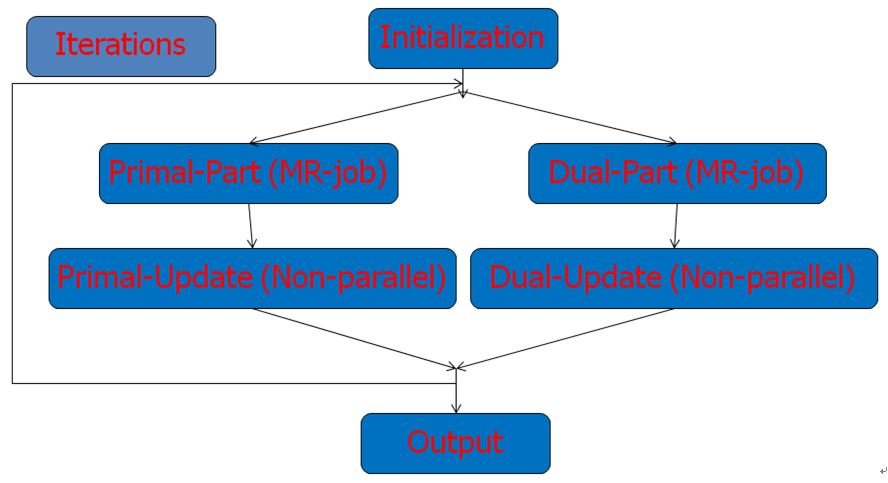
\includegraphics[height=3.5cm,width=6cm]{img/framework.png}
\caption{Parallel implementation flow chart for PSUBPLR-MR}
\end{figure}

For the parallelization period in the \textit{primal mapreduce job}, we take advantage of the MapReduce design that takes in every data instance in the training matrix.
Instead of the fashion in the sequential algorithm that we only sample a data instance in the primal update step, we compute gradients from "almost" all data instances and make the weighted average value according to vector $\bp$ as the output gradient for update.
The details of this algorithm design is shown in \textbf{Procedure Primal-Map(inputfile)} and \textbf{Procedure Primal-Reduce(key in, value in)}.
Here, we employ a randomization when we compute those "almost" all gradients.
As you can interpret from line 7 and 8 from \textbf{Procedure Primal-Map(inputfile)}, if $r=0$, then all data instances are computed.
As the expectation value for $\bp_t(i_t)$ is $\frac{1}{n}$, we normally set $r$ to range from 0 to 1.
For the parallelization period in the \textit{dual mapreduce job}, we actually implement an embarrassingly parallel operation.
It simply computes an individual value for each data instance in a parallel mode. It does not even need a reduce session.

There are also three more things that have to be addressed here.
First is the parameter passing issues. It critical to choose an efficient way to pass the updated parameters between iteration and even between different MapReduce jobs.
It is even more challenging when we have to deal with HDFS. It is clear that the fastest communication way is to pass parameters by \textit{Configuration()}.
However, it always has memory buffer size limits, and will greatly impair scalability when the number of parameters is huge.
Another way is to compress the parameter sequence in a string when sending and uncompress them when receiving. It has computational overhead and it still can not avoid the issue of memory buffer limit.
Thinking back on the philosophy of the design of Hadoop, the natural thing is to pass parameters by file, the same way to pass all the data.
We admit that it is inefficient, but it is the only way to support for large datasets.

The second issue is the small changes we make to cater for the $\ell_2$-penalty and $\ell_1$-penalty. The changes is only made in \textbf{Procedure PrimalUpdate}.
It does not affect little for the implementation, and the extension is just the same as that in \textbf{Algorithm SLLR}.
To have a brief and standard framework, we omit the explanation here.

The datasets are always sparse when data dimensionally is high. This makes us focus on dealing with data sparsity issue when writing code.
This is the third important thing for the algorithm, though it reflects nowhere from the pseudo-code.
Instead of naively writing the simple code for data intensive situations, we assign the index value for each data value in the sparse vector, and all computations are changed accordingly.
This gives us great efficiency improvement, and all results in section~\ref{sec:experiment} are using the code for sparsity.

\subsection{Parallel Sublinear algorithms in Spark}
The algorithm to solve sublinear learning for penalized logistic regression in Spark is shown below.
In the pseudo-code of Algorithm 3, Procedure for PrimalUpdate and Procedure for Dual-Map are the same as those in \textbf{Algorithm  PSUBPLR-MR}.
    \begin{table}[ht]
	\begin{tabular}{l}
    \hline\noalign{\smallskip}
	\textbf{Algorithm 3} PSUBPLR-SPARK \\
	\noalign{\smallskip}
	\hline
	\noalign{\smallskip}
    1:  ~Input parameters: $\varepsilon, \nu~or~\gamma, X, Y, n, d$ \\
    2:	~Initialize parameters: $T, \eta, {\mathbf{u}}_{0}, {\bw}_{1}, {\mathbf{\bq}}_{1}, {b}_{1}$\\
    3:  ~points $\leftarrow$ spark.textFile(inputfile).map(parsePoint()).cache() \\
    4:  ~Iterations: $t=1 \sim T$ \\
    5:  ~\tspace gradient $\leftarrow$ points.map($(\frac{1}{1+e^{-y((\bw_t^T \textbf{x})+b)}}-1) * y * \bp [index]$) \\
        ~~~\tspace\tspace\tspace\tspace\tspace .reduce(sum()) \\
    6:  ~\tspace ($\bw_{t+1}, b_{t+1}$)$\leftarrow$PrimalUpdate($\bw_t, b_t$) \\
    7:  ~\tspace Choose $j_t \leftarrow j$ with probability ${{\bw}_{t+1}\lj}^{2}/{\|{\bw}_{t+1}\|_2}^{2} $ \\
    8:  ~\tspace pAdjust $\leftarrow$ points.map(MW-Update()).reduce(copy()) \\
    9:  ~\tspace $\bp_{t+1}$$\leftarrow$DualUpdate($\bp_t$)  \\
    10: \textbf{Output}($\bw, b$) \\
    \hline
    \end{tabular}
	\end{table}

This parallel design is very similar to that of \textbf{Algorithm  PSUBPLR-MR}.
The most important difference is the \textit{cache()} operation in line 3.
To make it work in Spark, we follow the rules to construct an RDD for each data instance.
Also to cater for data sparsity, the design is the every data value correspond to its individual index. And the index also participate in the computation along with the value.
We also omit the changes for $\ell_2$-penalty and $\ell_1$-penalty here to make the algorithm easier to be understood.

We can now study the running time of parallel sublinear method for LR.
In parallel mode, the primal update contains an update of $w_t$, which takes $O(n)$ time.
And the dual update contains a $\ell_2$-sampling process for the choice of $j_t$ in $O(d)$ time, and an update of $\bp$ in $O(1)$ time.
Altogether, each iteration takes $O(n+d)$ time, which is sublinear to the dataset size.
Compared to the analysis of sequential algorithm, parallelization does not change computational complexity.
However, by reducing the constant coefficient from 2 to 1 in each iteration, it can be two times faster than sequential sublinear algorithm theoretically.
Moreover, by starting two separate MapReduce jobs in a iteration simultaneously, the running time can be reduced to $O(max\{n,d\})$.

\subsection{Parallel Gradient Descent in Spark}
The parallel gradient descent method to solve LR in Spark is shown below.
    \begin{table}[ht]
	\begin{tabular}{l}
    \hline\noalign{\smallskip}
	\textbf{Algorithm 4} PGDPLR-SPARK \\
	\noalign{\smallskip}
	\hline
	\noalign{\smallskip}
    1:  Input parameters: $\varepsilon, \nu~or~\gamma, X, Y, n, d$ \\
    2:	Initialize parameters: $T, \eta, {\mathbf{u}}_{0}, {\bw}_{1}, {\mathbf{\bq}}_{1}, {b}_{1}$\\
    3:  points $\leftarrow$ spark.textFile(inputfile).map(parsePoint()).cache() \\
    4:  Iterations: $t=1 \sim T$ \\
    5:  \tspace gradient $\leftarrow$ points.map($(\frac{1}{1+e^{-y((\bw_t^T \textbf{x})+b)}}-1)*y$) \\
        ~~\tspace\tspace\tspace\tspace\tspace .reduce(sum()) \\
    6:  \tspace $\bw_{t+1} = \bw_t - gradient * \textbf{x}$ \\
    7:  \tspace $b = b - gradient$ \\
    8:  \textbf{Output}($\bw, b$) \\
    \hline
    \end{tabular}
	\end{table}

In the pseudo-code of Algorithm 4, we can find that it is implemented in an embarrassingly parallel mode.
We can take in all the data at the same iteration and just compute the gradient in a MapReduce fashion.
As for the \textit{cache()} operation and RDD design for data sparsity, it is the same as \textbf{Algorithm PSUBPLR-SPARK}.

\subsection{Online Stochastic Gradient Descent in Mahout}
Though SGD is an inherently sequential algorithm, it is blazingly fast and thus it is not a problem for Mahout's implementation to handle training sets of tens of millions of examples.
With the down-sampling typical in many datasets, this is equivalent to a dataset with billions of raw training examples.
The SGD system in Mahout is an online learning algorithm which means that you can learn models in an incremental fashion and that we can do performance testing as your system runs.
This also means that we can stop training when a model reaches a target level of performance.
The SGD framework includes classes to do online evaluation using cross validation (the \textit{CrossFoldLearner}) and an evolutionary system to do learning hyper-parameter optimization on the fly (the \textit{AdaptiveLogisticRegression}).
The \textit{AdaptiveLogisticRegression} system makes heavy use of threads to increase machine utilization.
The way it works is that it runs 20 \textit{CrossFoldLearners} in separate threads, each with slightly different learning parameters.
As better settings are found, these new settings are propagating to the other learners.

Because the SGD algorithms need to have fixed length feature vectors and because it is a pain to build a dictionary ahead of time, most SGD applications use the hashed feature vector encoding system that is rooted at \textit{FeatureVectorEncoder}.
The basic idea is that you create a vector, typically a \textit{RandomAccessSparseVector}, and then you use various feature encoders to progressively add features to that vector.
The size of the vector should be large enough to avoid feature collisions as features are hashed.
There are specialized encoders for a variety of data types.
You can normally encode either a string representation of the value you want to encode or you can encode a byte level representation to avoid string conversion.
In the case of \textit{ContinuousValueEncoder} and \textit{ConstantValueEncoder}, it is also possible to encode a null value and pass the real value in as a weight.

In our implementation, we use \textit{RandomAccessSparseVector} for data sparsity and the function call by \textit{OnlineLogisticRegression} to train.
We also do the cross validation part. However, to be synchronized with other methods, we write our own code to do cross validation.
	
\section{Experiments Setup} \label{sec:setup}
In this section, we explains details of the datasets information, cluster information, and the test programs of our experiments.

\subsection{Datasets Information}
We choose five open datasets to run all six test programs:	
The	Simulated \textbf{2d} dataset has 2 features and 200 instances.
The	\textbf{20NewsGroup} dataset has 16428 features and 1988 instances. We split it into a training set of 1800 instances and a test set of 188 instances.	
The	third test dataset is the \textbf{Gisette}~\cite{guyon2004result} dataset, which has 5000 features and 7000 instances. We split it into a training set of 6000 instances and a test set of 1000 instances.
The	fourth test dataset is the \textbf{ECUESpam}~\cite{DelanyKBS05} dataset, which has 100249 features and 10678 instances (after proper preprocessing). We split it into a training set of 9000 instances and a test set of 1687 instances.
Finally, we have the \textbf{URL-Reputation}~\cite{ma2009identifying} dataset, which has 3231961 features and 2376130 instances.
We split it into a training set of 2356130 instances and a test set of 20000 instances.
Apart from the Simulated \textbf{2d} dataset, other four datasets are all sparse. Details are shown in Table~\ref{tab:table1}.
We randomly repeat such split 20 times and our analysis is based on the average performance of 20 repetitions.

In Table~\ref{tab:table1}, \textit{Density} is computed as
\[
Density(Dataset)~=~\frac{\#~of~Nonzeros}{Total~\#~of~entries},
\]
which is adopted from~\cite{sarwar2001item}.
\textit{Balance} describes the binary distribution of labels.
We compute it as following:
\[
Balance(Dataset)~=~\frac{\#~of~Positive~Instances}{\#~of~Negative~Instances}.
\]
\begin{table}[h]
\centering
\caption{Datasets}\label{tab:table1}
\begin{tabular}{|c|c|c|c|c|c|}
\hline
    Name           & $n$ & $d$ & Density & Nonzeros & Balance \\
\hline
    2d             & 2             & 200            & 1.0                  & 400                 & 1.000 \\
\hline
    20NewsGroup    & 16428         & 1988           & $7.384\times10^{-3}$ & 238511              & 1.006 \\
\hline
    Gisette        & 5000          & 7000           & 0.12998              & 4549319             & 1.000 \\
\hline
    ECUESpam       & 100249        & 10687          & $2.563\times10^{-3}$ & 2746159             & 5.882 \\
\hline
    URL-Reputation & 3231961       & 2376130        & $3.608\times10^{-5}$ & 277058644           & 0.500 \\
\hline
\end{tabular}
\end{table}
We carefully select these five datasets.
The Simulated \textbf{2d} dataset can be viewed for visual result and serves for initial test of correctness of implementation.
The \textbf{20NewsGroup} dataset is best-known for the test of LR model, which has a balanced distribution between positive and negative data instances.
The \textbf{Gisette} dataset is relatively larger, and data is less sparse. Thus it requires more computation theoretically.
The \textbf{ECUESpam} dataset features for its inbalanced distribution between positive and negative data instances. It has a higher data dimensionality than textbf{Gisette} dataset. However, because of data sparsity, it has fewer nonzero values involved in the computation.
Finally, the \textbf{URL-Reputation} dataset contains millions of data instances and features. The raw data is stored in the svmlight format, which has the size of more than 2GB. It achieves the current level for massive dataset, and exceed the scalability of Liblinear, which will be shown below.

\subsection{Cluster Information}
The cluster that we implement on has the following configurations shown in Table~\ref{tab:table2}.
\begin{table}[h]
\centering
\caption{Cluster Information}\label{tab:table2}
\begin{tabular}{|c|c|}
\hline
    CPU Model & Intel Xeon E5-1410: 2.80GHz \\
\hline
    Number of node & 6 \\
\hline
    Number of CPU per node & 4 Cores, 8 Threads \\
\hline
    RAM per node & 16G \\
\hline
    Disk per node & 4T HDD\\
\hline
    Interconnection Method & Gigabyte Ethernet  \\
\hline
\end{tabular}
\end{table}
This kind of cluster configuration is now more and more common in research labs. Hence our results reported in the following can have a real impact in the research community.

\subsection{Test Programs}
There are all together 6 test programs for comparison.
Online stochastic gradient descent method is run on Mahout in a sequential mode.
Liblinear~\cite{fan2008liblinear} is the baseline test program we choose. It is sequential and it outperforms many other programs for LR on a single machine.
SLLR performs sequential sublinear algorithm on a single machine.
PSUBPLR-MR performs parallel sublinear algorithm on Hadoop on cluster.
PGDPLR-SPARK is the test program for parallel gradient descent run on Spark.
PSUBPLR-SPARK implements parallel sublinear algorithm run on Spark.

\section{Experimental Results} \label{sec:experiment}
In this section, we conduct an empirical analysis of our algorithms.

\subsection{Results on Simulated 2d Dataset}
\begin{figure}[tb] \label{fig:02}
\center 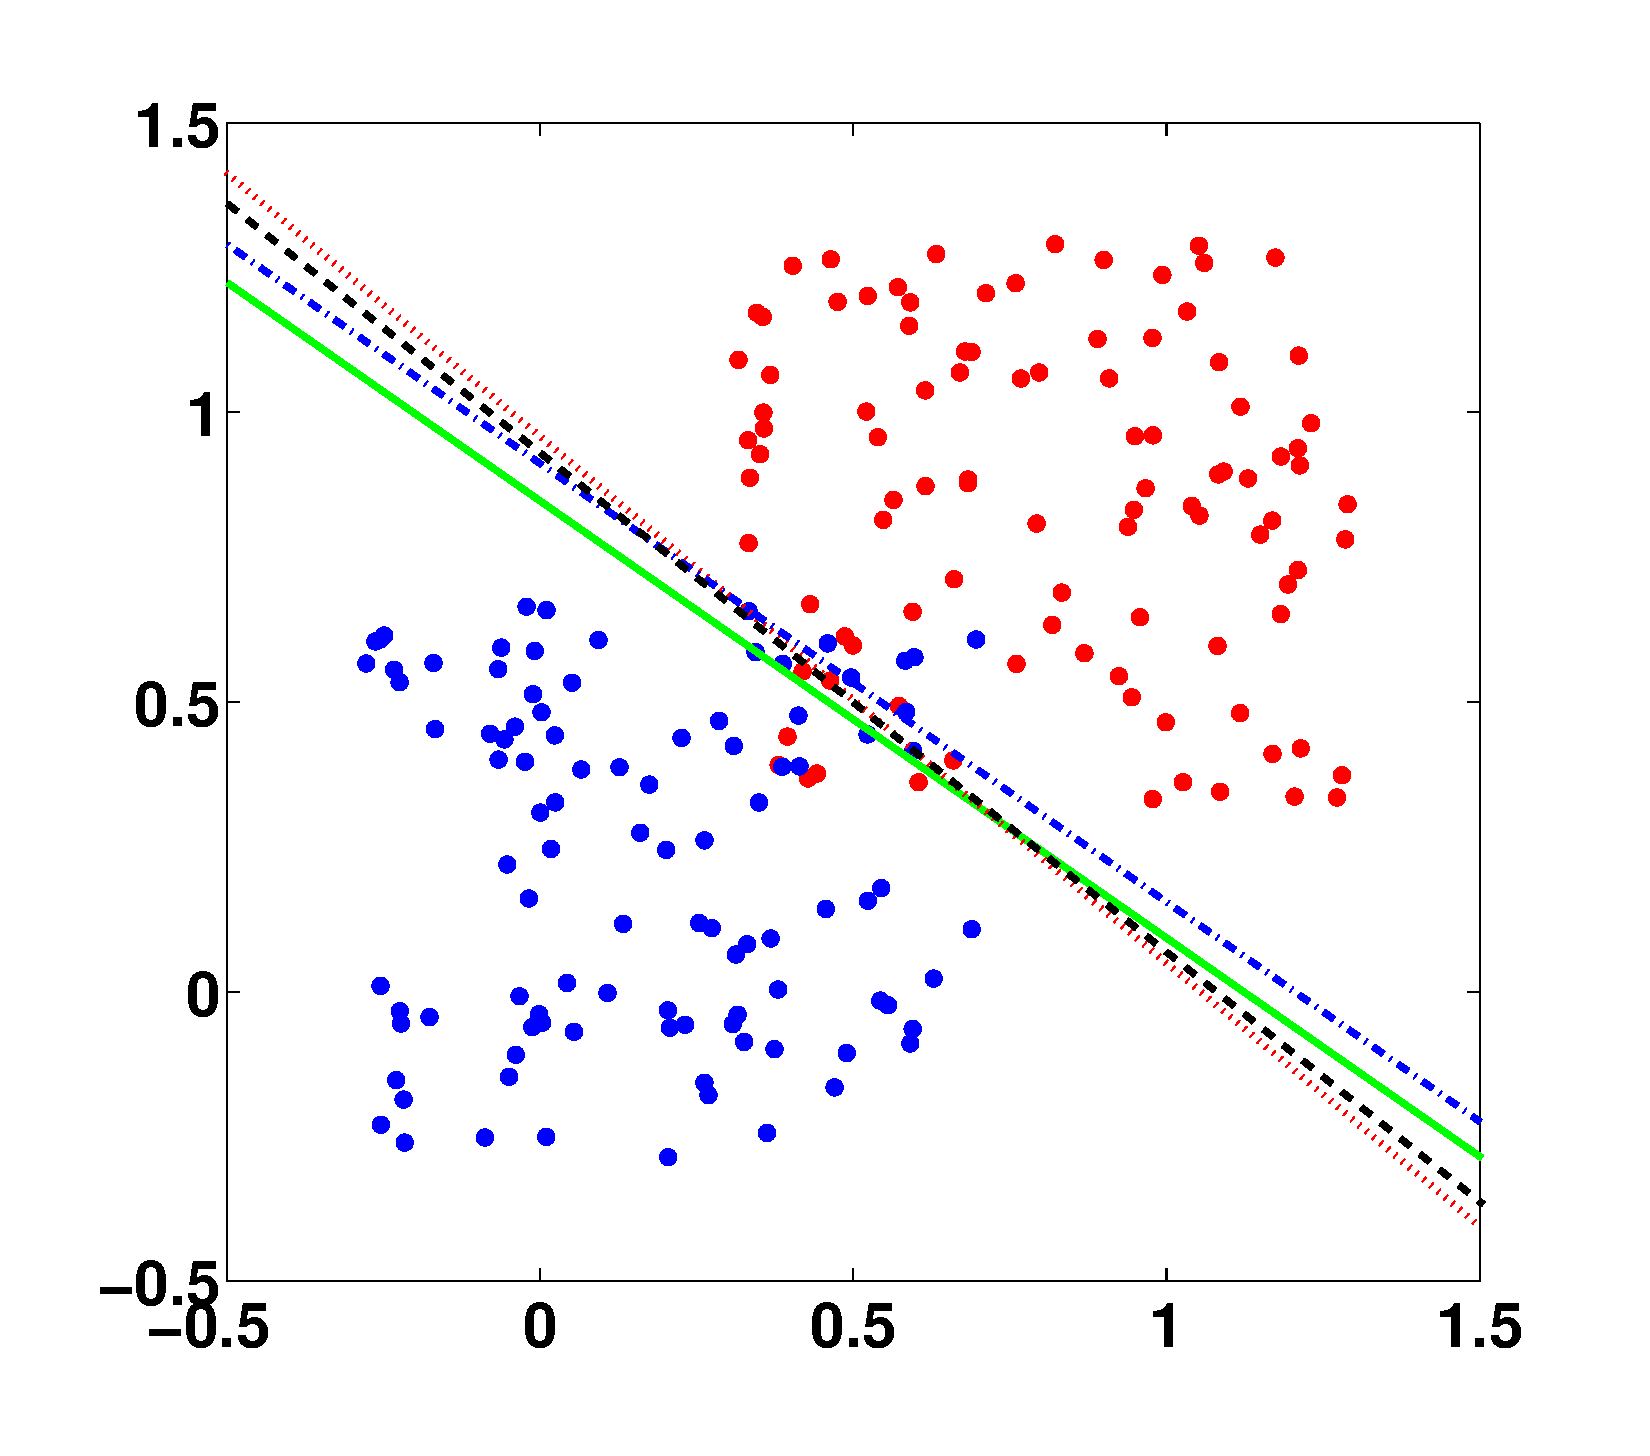
\includegraphics[height=5cm,width=6cm]{img/2d-show.eps}
\caption{Visual Result on Simulated \textbf{2d} Dataset}
\end{figure}
Fig.~\ref{fig:02} shows the visual result for Simulated \textbf{2d} Dataset.
Here we use all data for training and testing, thus "Test Error" here can be interpreted as "Training Error".
The blue line represents the learned separation vector of Mahout.
The black line indicates the result for Liblinear.
The green line shows the result for all sublinear methods, including SLLR, PSUBPLR-MR and PSUBPLR-SPARK.
The red line is the result for PGDPLR-SPARK.
The results on the Simulated \textbf{2d} Dataset proves the correctness of all test programs.

\subsection{Results on Precision} \label{sec:precision}
\begin{table}[h]
\centering
\caption{Accuracy Results}\label{tab:table3}
\begin{tabular}{|c|c|c|c|c|c|}
\hline
           & 2d   & 20NewsGroup & Gisette & ECUESpam & URL-Reputation \\
\hline
Mahout     & 93.5\% & 71.3\% & 91.5\% & 85.2\% & 91.5\% \\
\hline
Liblinear  & 93.0\% & 92.0\% & 97.4\% & 97.1\% & \XSolid \\
\hline
SLLR       & 93.5\% & 91.5\% & 94.8\% & 92.3\% & 94.2\% \\
\hline
PSUBPLR-MR & 93.5\% & 90.5\% & 94.6\% & 91.7\% & 93.8\% \\
\hline
PGDPLR-SPARK & 93.5\% & 92.0\% & 97.0\% & 93.7\% & 96.0\% \\
\hline
PSUBPLR-SPARK & 93.5\% & 90.5\% & 95.8\% & 91.7\% & 94.0\% \\
\hline
\end{tabular}
\end{table}
Accuracy of six test programs achieved on five datasets are shown in Table~\ref{tab:table3}. These are averaged results of cross validation.
From Fig.~\ref{fig:03} to Fig.~\ref{fig:07}, we show the test error as a function of iteration number on each dataset for all six test programs.
Note that, Liblinear can not be fully implemented the \textbf{URL-Reputation} dataset on our machine due to memory limit.
This proves the scalability issue of Liblinear.

\begin{figure}[tb] \label{fig:03}
\center 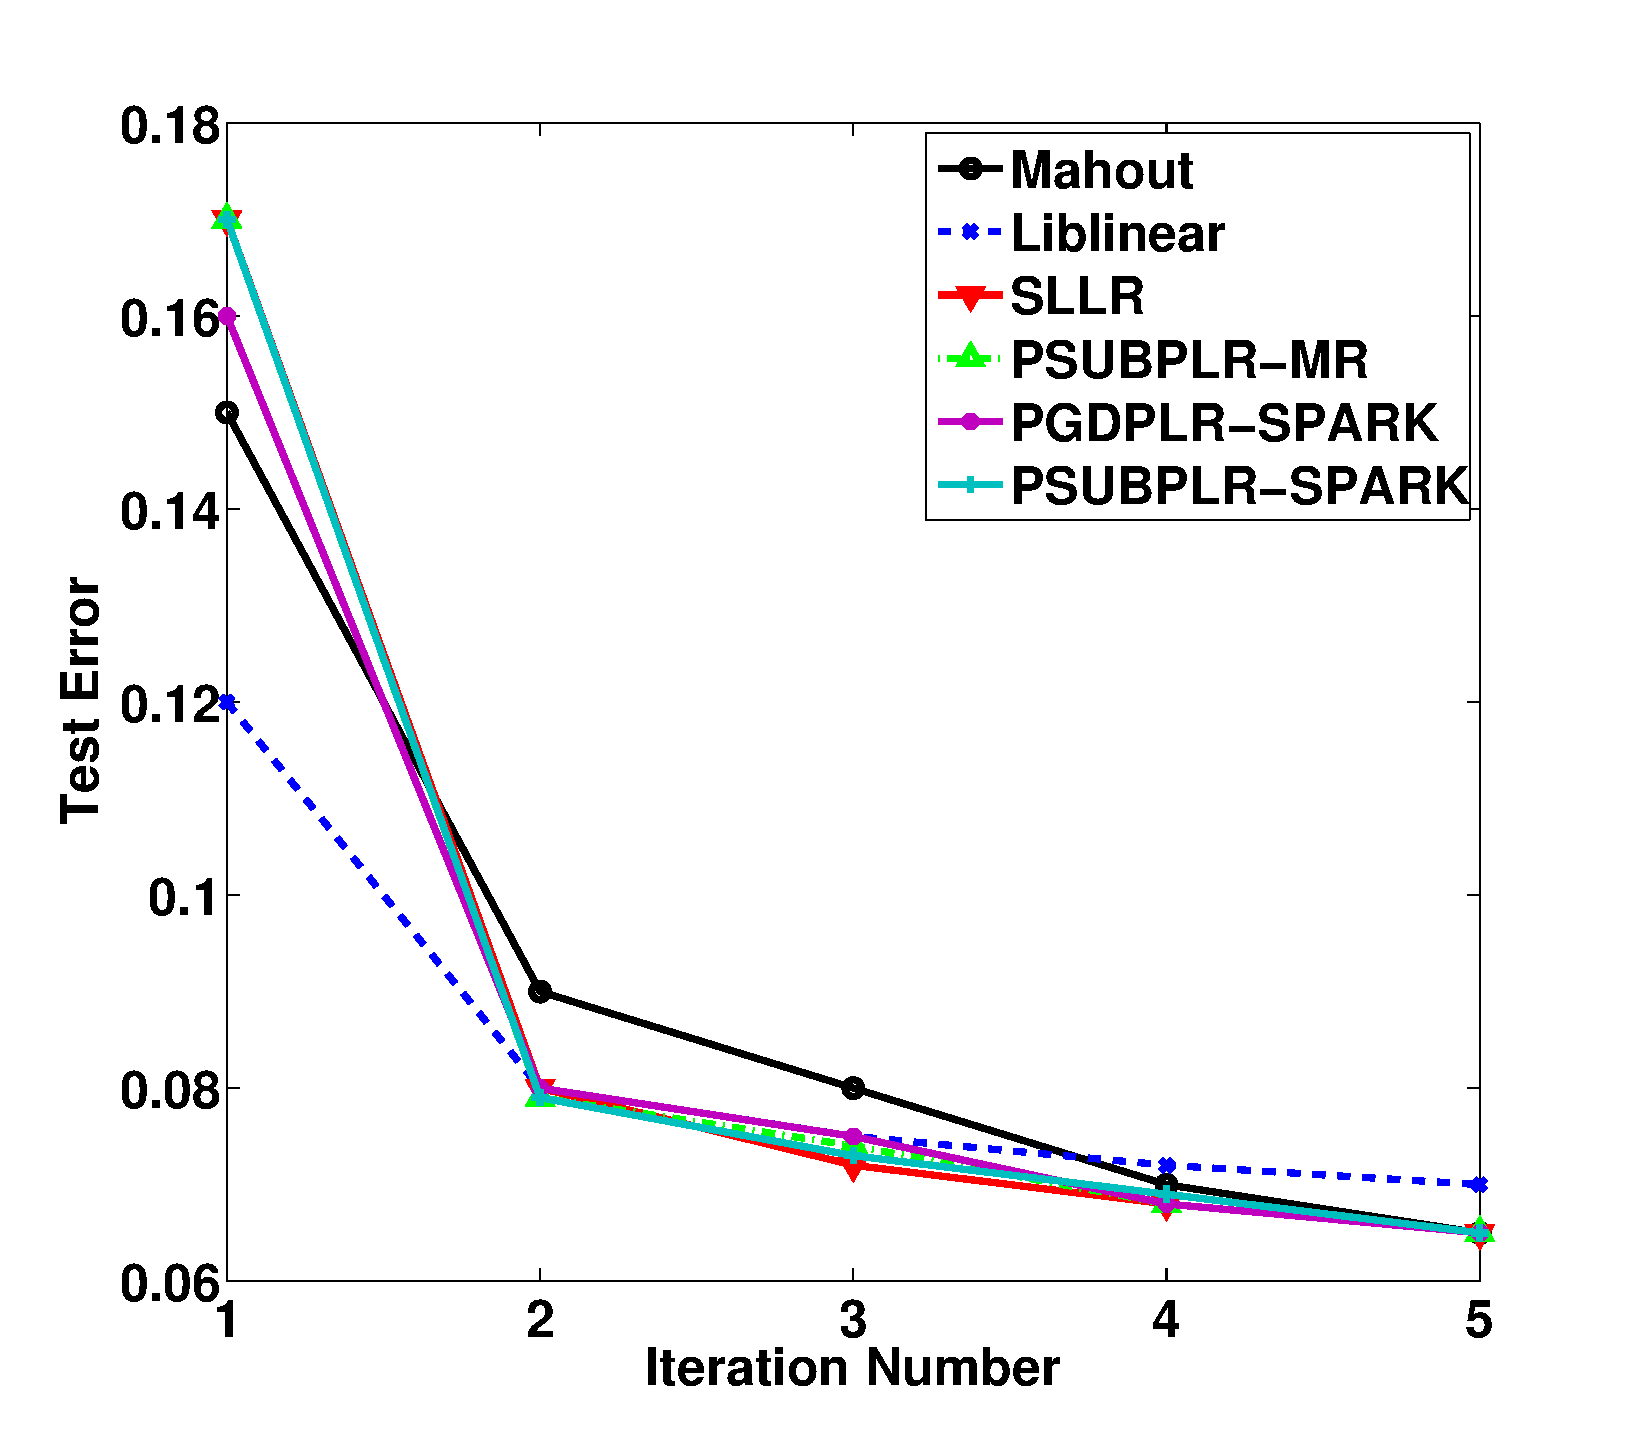
\includegraphics[height=4.5cm,width=5cm]{img/2d_accuracy_iteration.eps}
\caption{Test error, as a function of iteration number on Simulated \textbf{2d} Dataset}
\end{figure}

\begin{figure}[tb] \label{fig:04}
\center 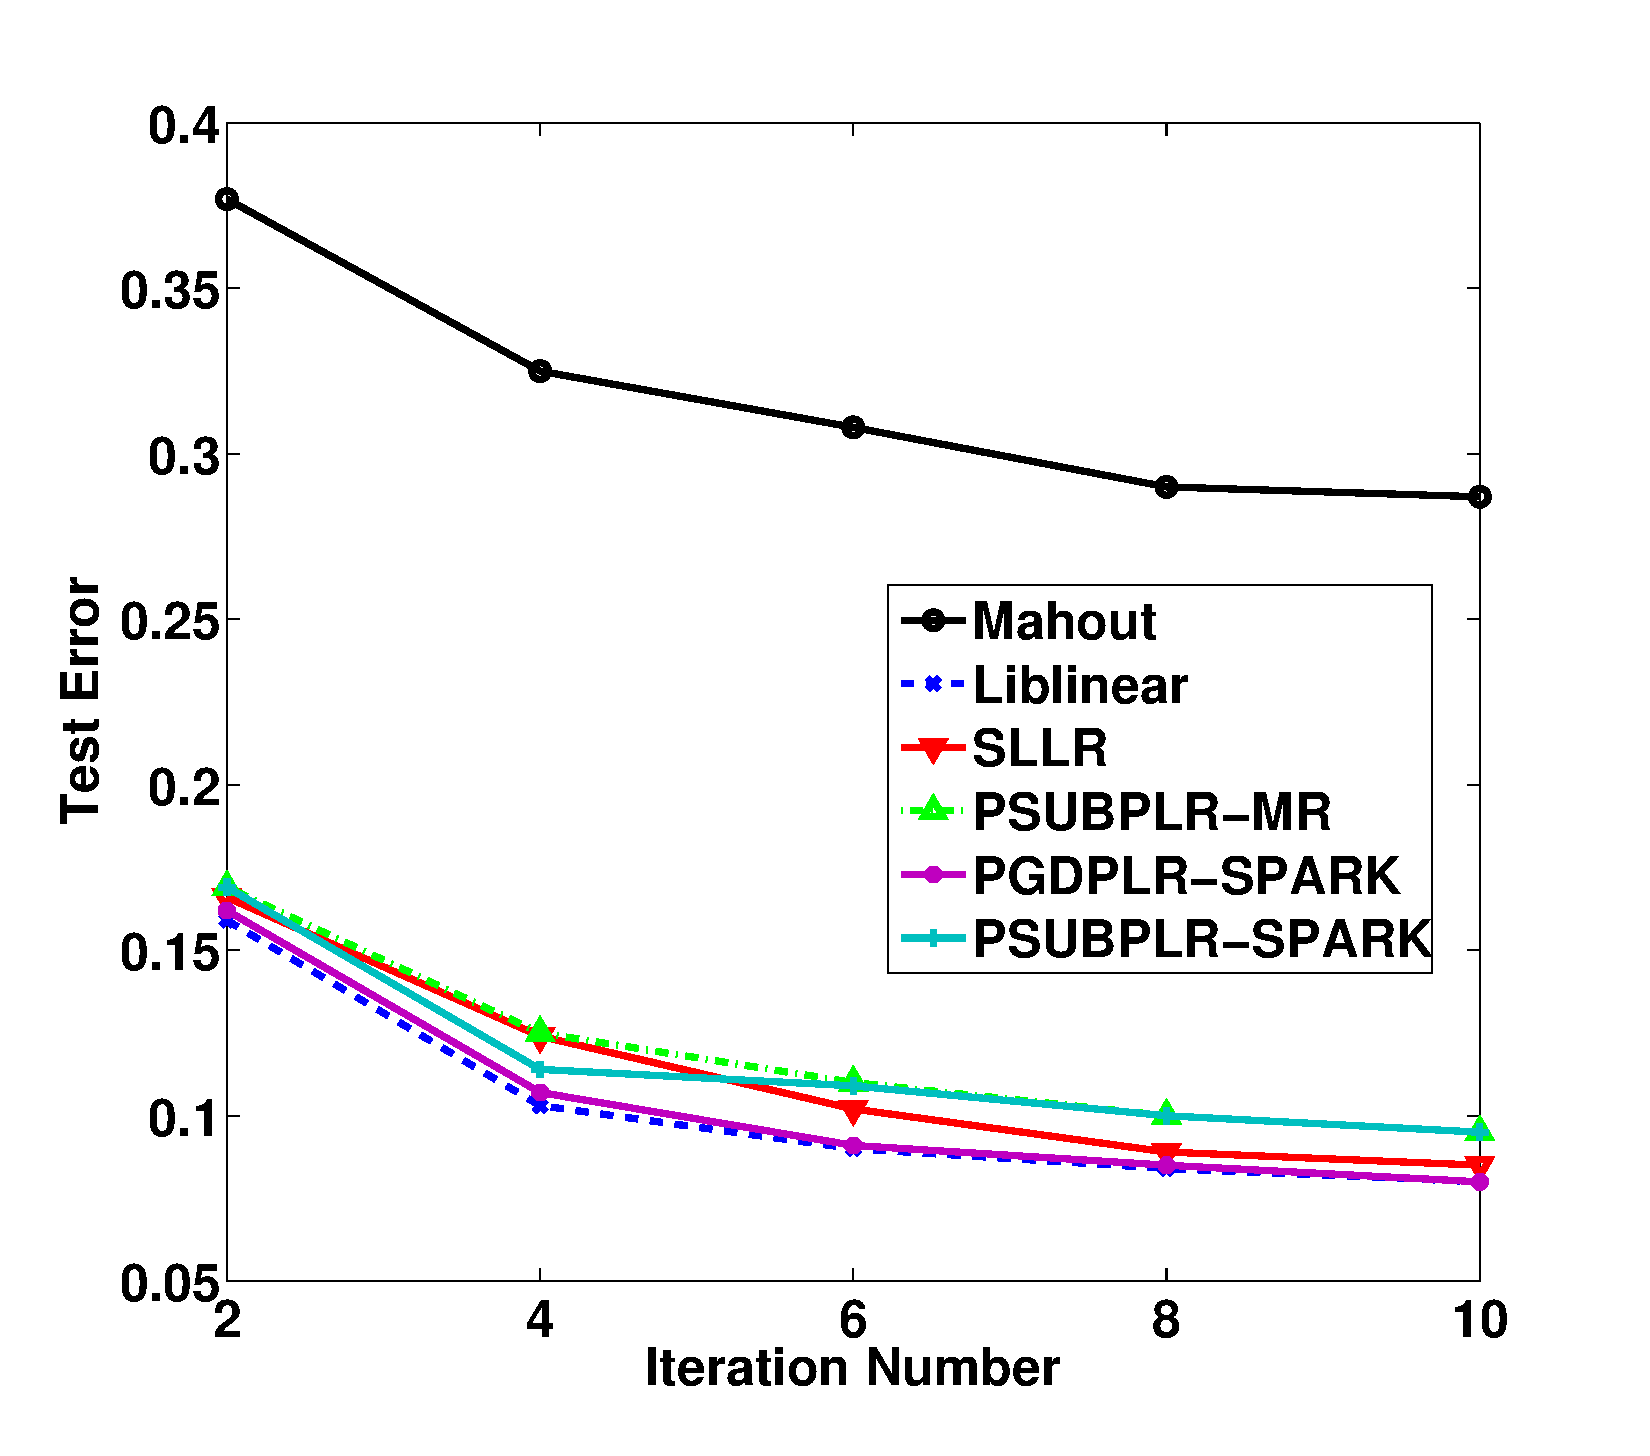
\includegraphics[height=4.5cm,width=5cm]{img/20NewsGroup_accuracy_iteration.eps}
\caption{Test error, as a function of iteration number on \textbf{20NewsGroup} Dataset}
\end{figure}

\begin{figure}[tb] \label{fig:05}
\center 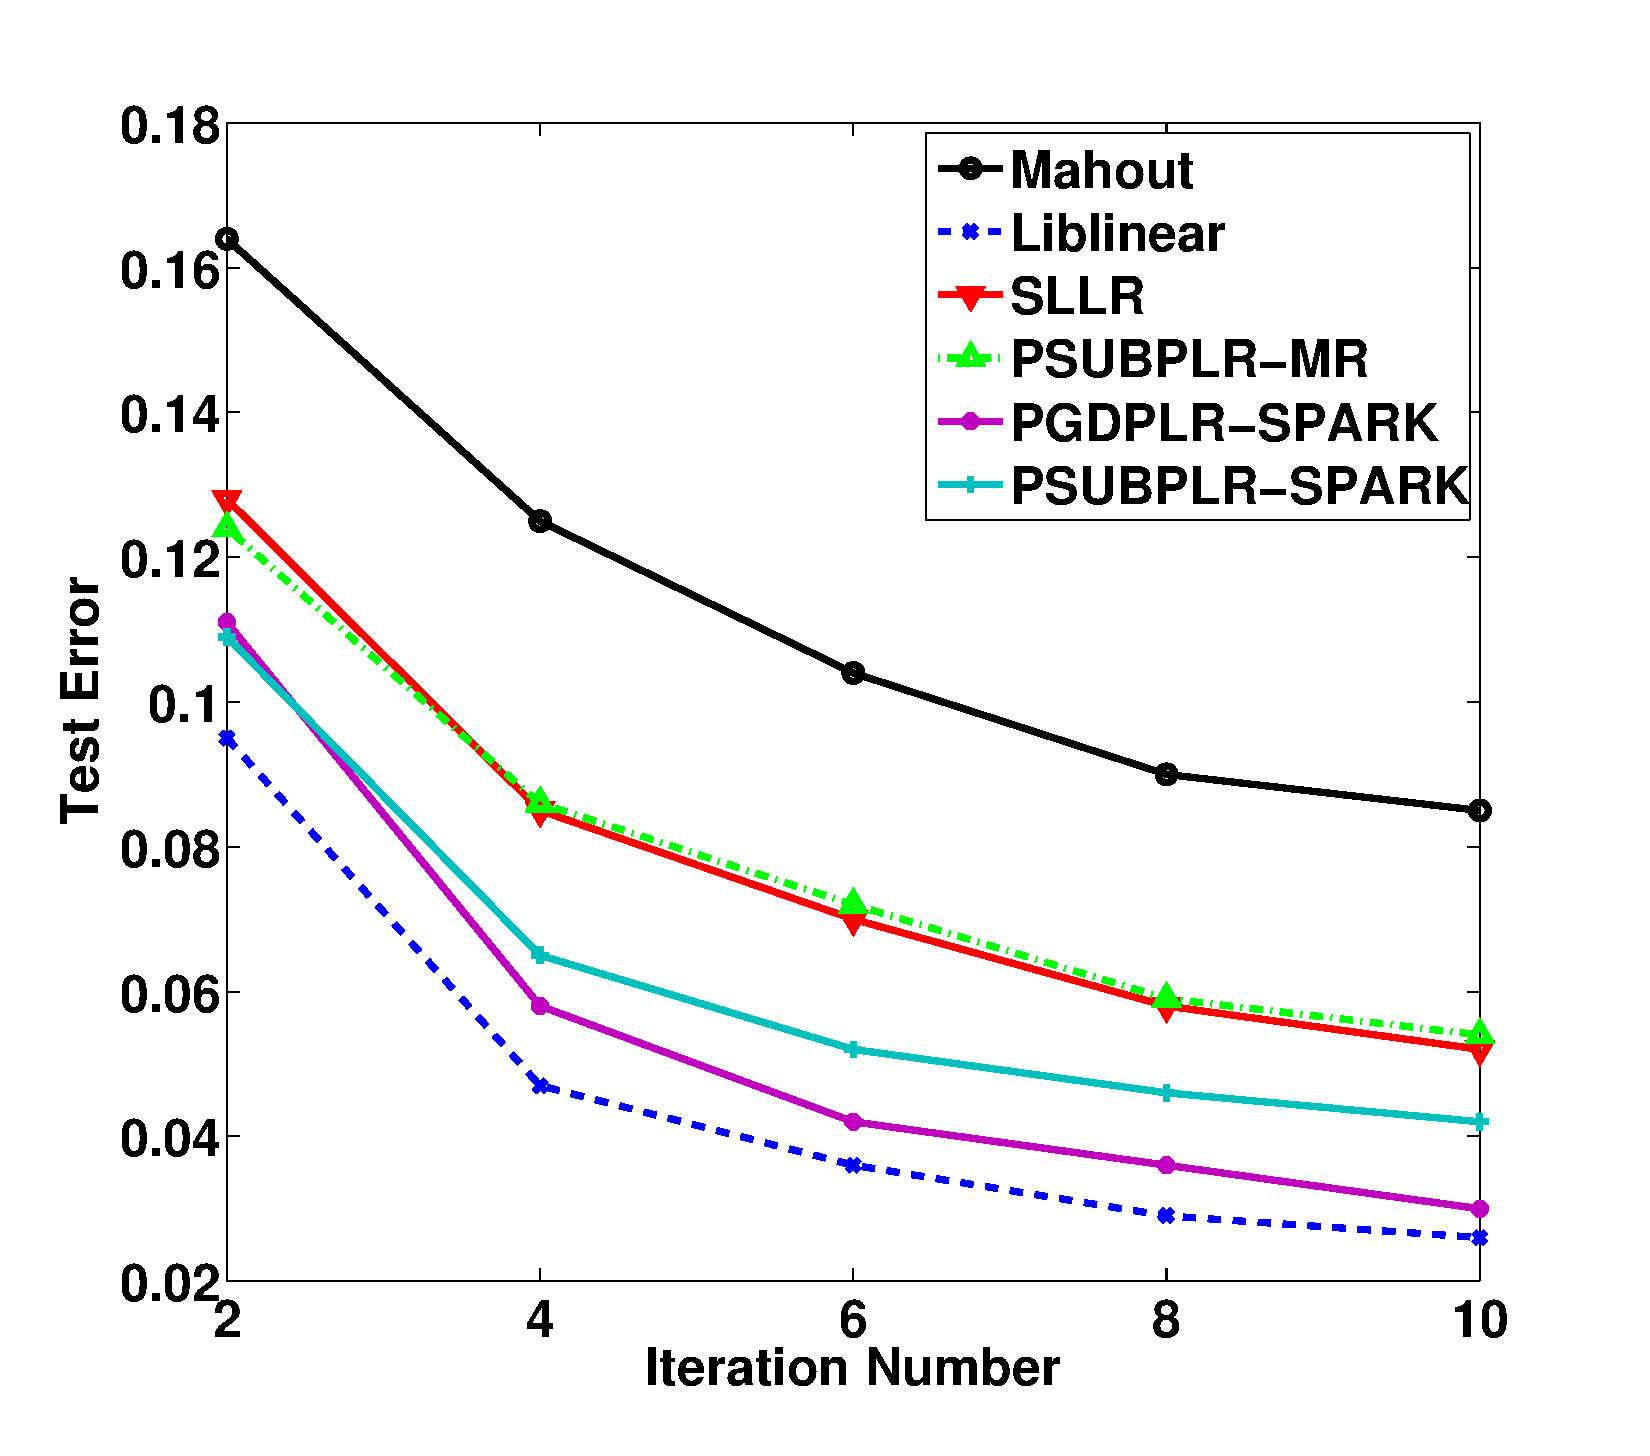
\includegraphics[height=4.5cm,width=5cm]{img/Gisette_accuracy_iteration.eps}
\caption{Test error, as a function of iteration number on \textbf{Gisette} Dataset}
\end{figure}

\begin{figure}[tb] \label{fig:06}
\center 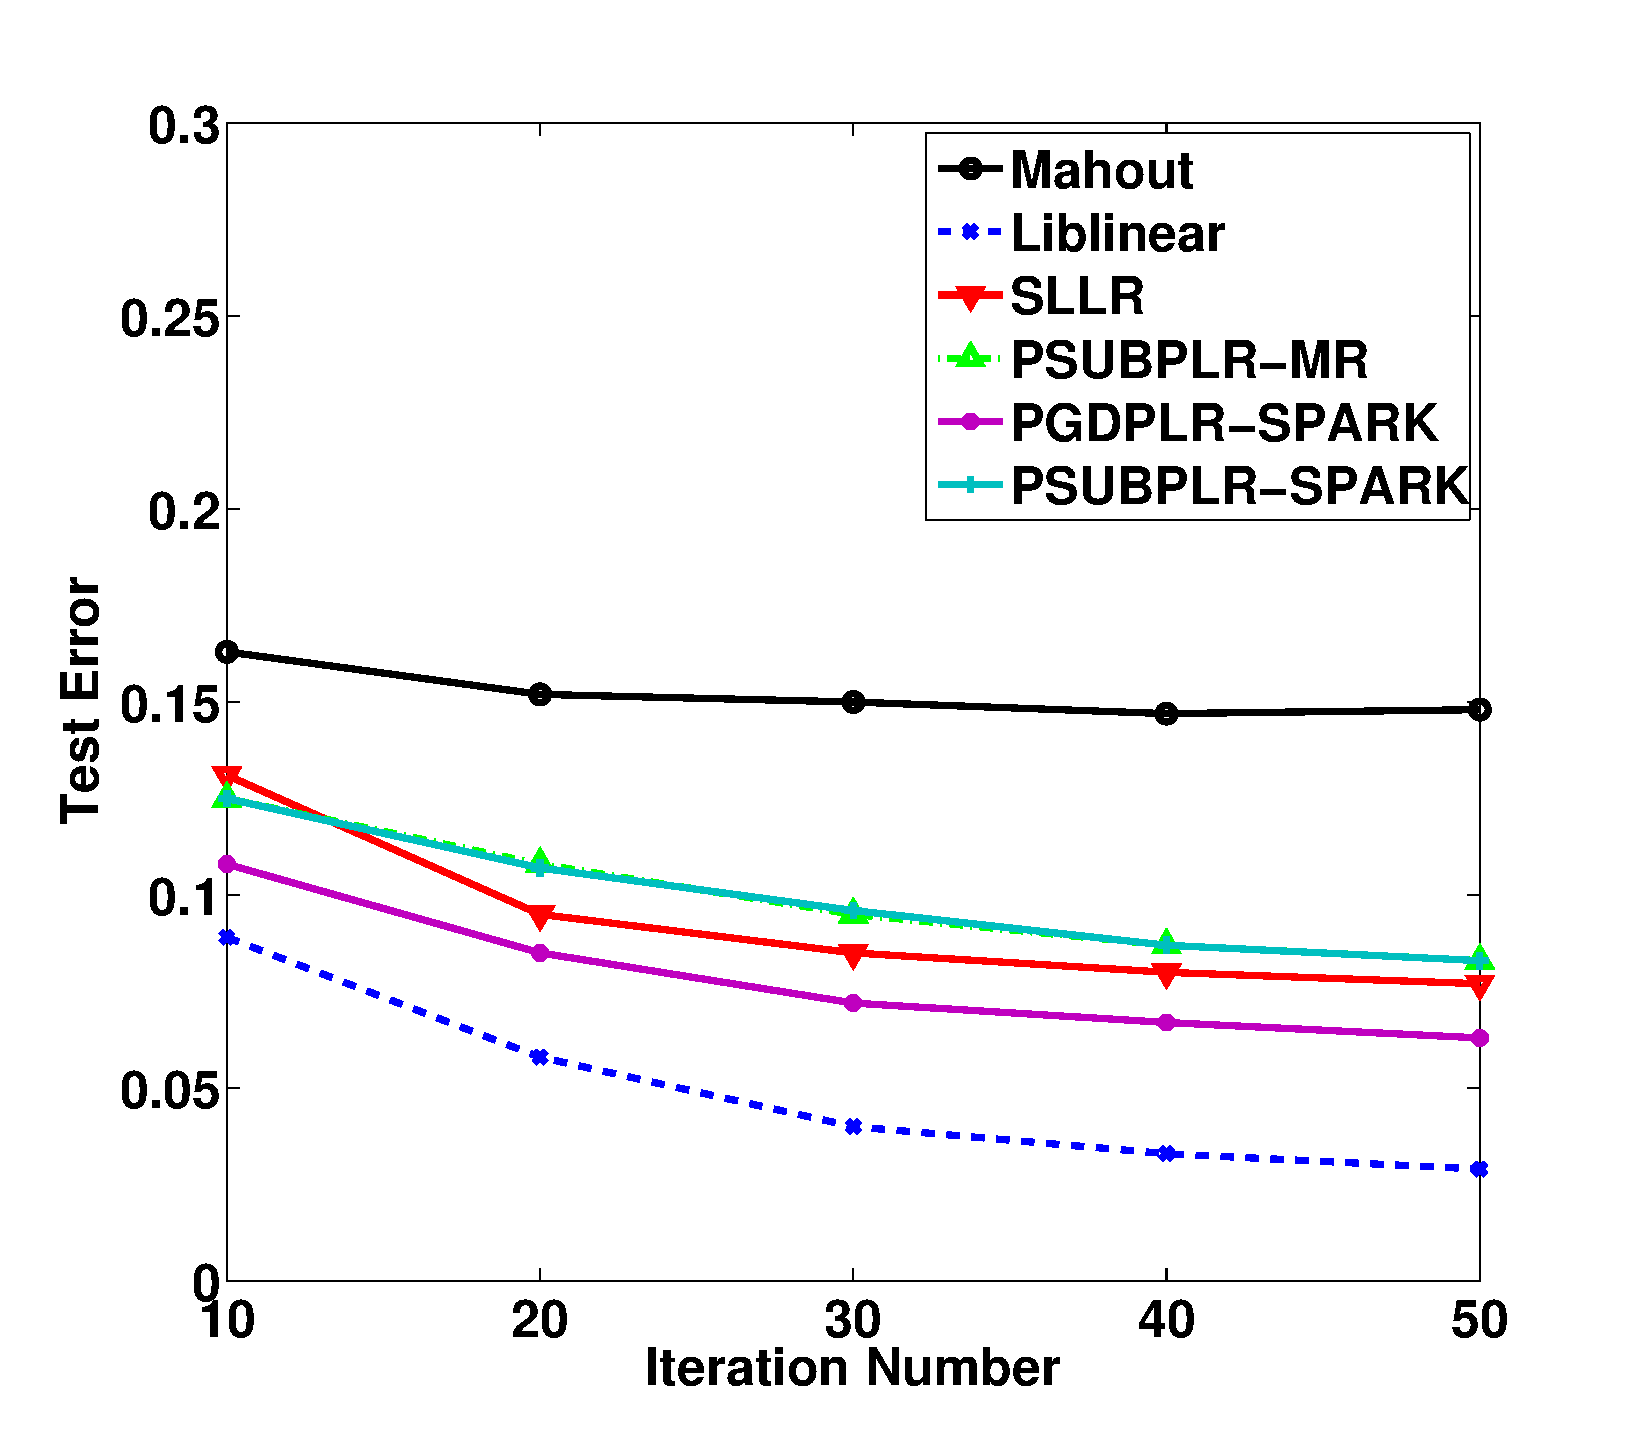
\includegraphics[height=4.5cm,width=5cm]{img/ECUESpam_accuracy_iteration.eps}
\caption{Test error, as a function of iteration number on \textbf{ECUESpam} Dataset}
\end{figure}

\begin{figure}[tb] \label{fig:07}
\center 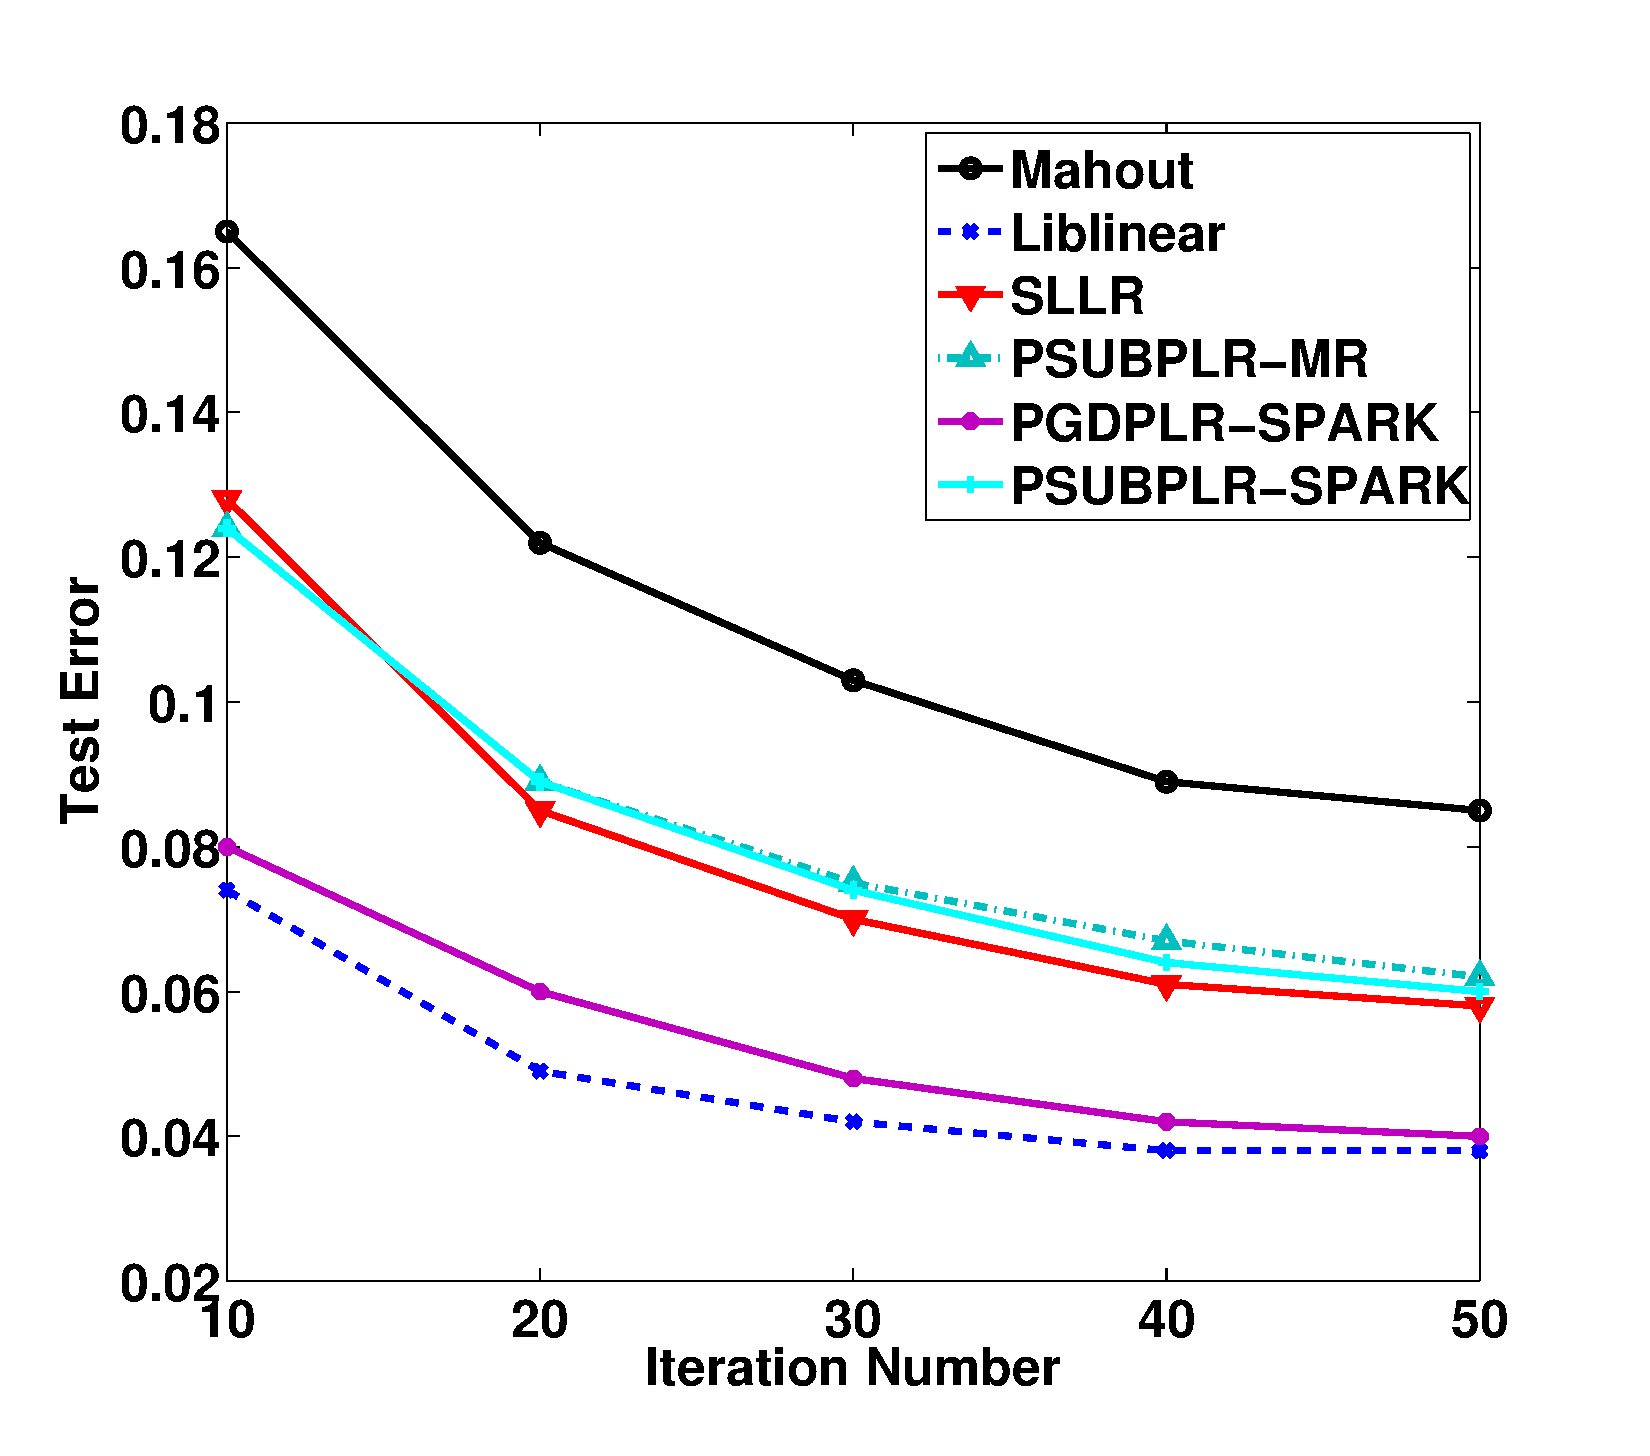
\includegraphics[height=4.5cm,width=5cm]{img/URL-Reputation_accuracy_iteration.eps}
\caption{Test error, as a function of iteration number on \textbf{URL-Reputation} Dataset}
\end{figure}

\subsection{Results on Running Time} \label{sec:time}
\begin{table}[h]
\centering
\caption{Running Time Results}\label{tab:table4}
\begin{tabular}{|c|c|c|c|c|c|}
\hline
           & 2d   & 20NewsGroup & Gisette & ECUESpam & URL-Reputation \\
\hline
Mahout     & 0.595s & 9.827s & 131.807s & 96.611s & 10100.209s \\
\hline
Liblinear  & 0.078s & 0.793s & 2.364s & 13.161s & \XSolid \\
\hline
SLLR       & 1.761s & 20.046s & 130.451s & 1028.185s & 3248.473s \\
\hline
PSUBPLR-MR & 120.186s & 1360.854s & 3687.941s & 11478.706s & 16098.260s \\
\hline
PGDPLR-SPARK & 0.681s & 10.517s & 99.156s & 924.020s & 3615.780s \\
\hline
PSUBPLR-SPARK & 1.325s & 8.571s & 89.094s & 796.802s & 2918.470s \\
\hline
\end{tabular}
\end{table}
Running Time of six test programs used on five datasets are shown in Table~\ref{tab:table4}.
These are averaged results corresponding to the accuracy we achieved in Table~\ref{tab:table3}.

\begin{figure}[tb] \label{fig:08}
\center 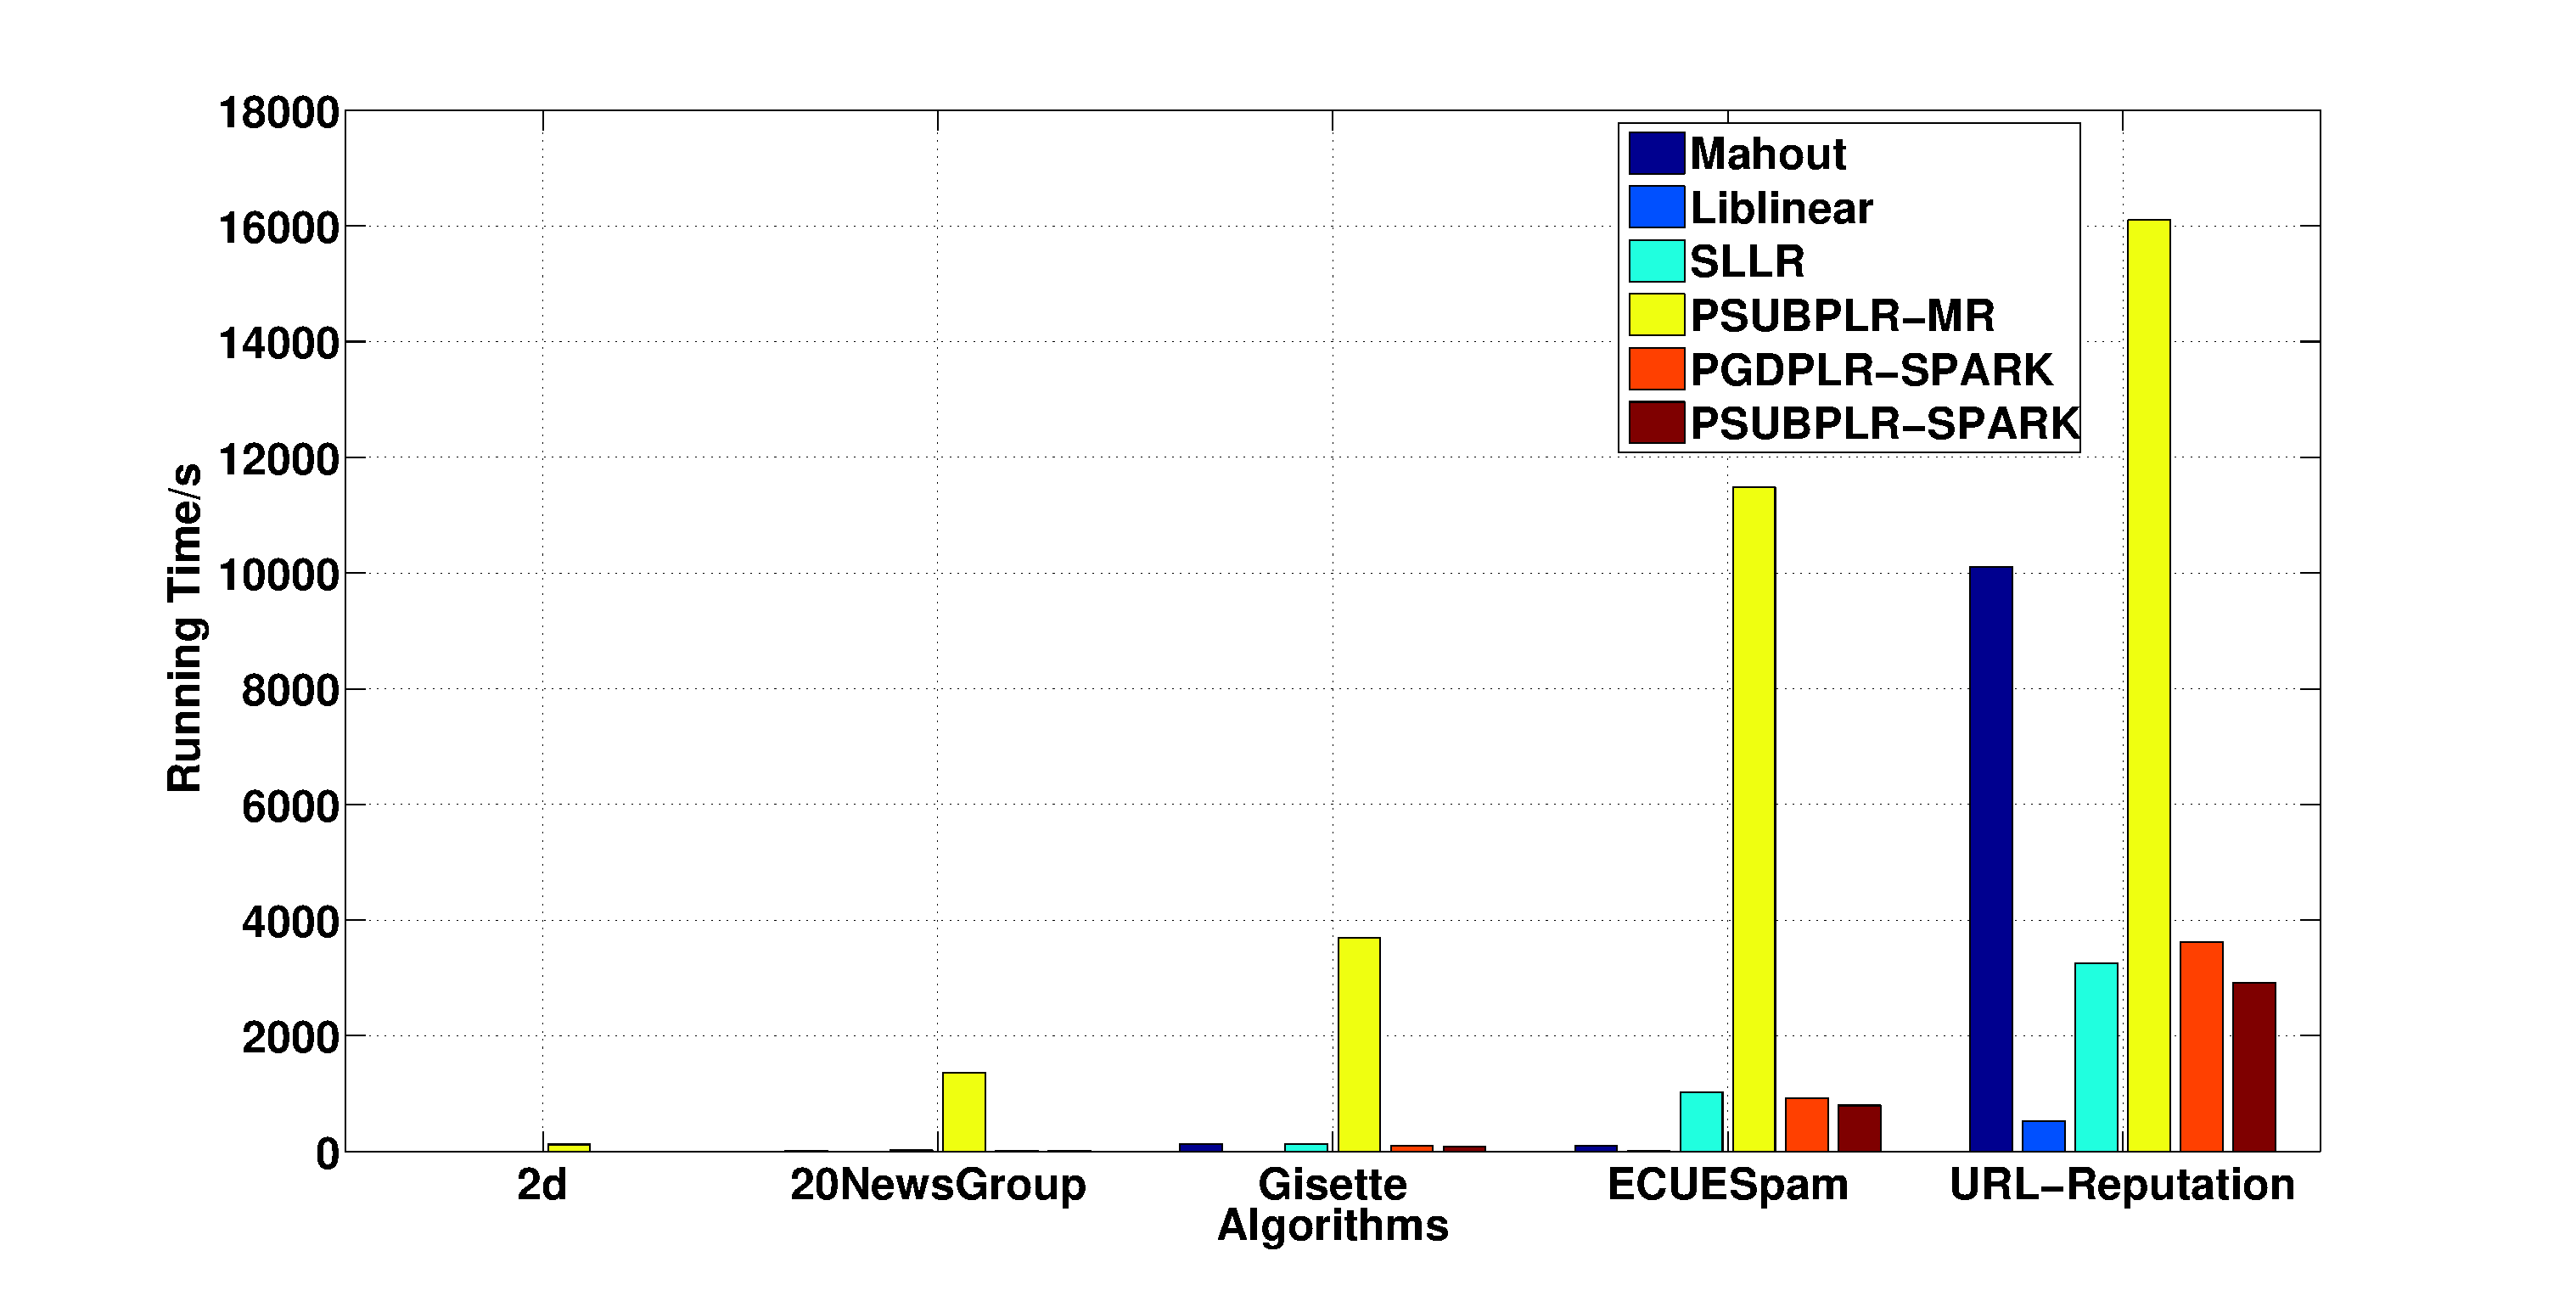
\includegraphics[height=4.5cm,width=9cm]{img/all_time.eps}
\caption{All running times}
\end{figure}
In another way, we show the running time results in Fig.~\ref{fig:08} for comparison.

From the accuracy results in section~\ref{sec:precision} and running time results in section~\ref{sec:time}.
We can come up with following conclusions.
\begin{enumerate}
    \item Liblinear always performs the best. It fully utilizes memory and single machine implementation does not require any communication between machines, which causes overhead.
          However, its scalability is limited by the memory size of the single machine that it runs on. This prevents its use in massive datasets.
          Nevertheless, if the dataset can be fully loaded into a single machine's memory, this efficient and direct sequential way of implementation is still recommended.
    \item Mahout's precision is not good, especially for those datasets in which positive and negative instances are not balanced.
          However, it is a representative of sequential algorithm that can train massive data in acceptable time.
          When we monitor its memory when running, it is much lower than Liblinear. This is the advantage brought by both online algorithm and hashing operations on features.
          Thus, it provides good scalability guarantee. If you are in the situation of single machine and limited memory, sequential online training like Mahout is recommended.
    \item The precision of all sublinear methods is acceptable. The developed parallel sublinear algorithm only has a small drop in precision.
    \item Hadoop system has a great drawback for running LR optimization methods. Its cluster programming model is based on acyclic data flow from stable storage to stable storage.
          Though it has the benefits of deciding where to run tasks and can automatically recover from failures in runtime, acyclic data flow is inefficient for iterative algorithms.
          All six test programs contains a number of iterations, thus making PSUBPLR-MR performs poorly, even worse than sequential algorithms.
          When we study the details of Hadoop implementation, we find the MapReduce job starting time in PSUBPLR-MR is about 20s. It consists of task configuration time and parameter passing time.
          This running time overhead is not negligible, especially when dataset is relatively small.
          We also identify the running of "Primal-Map" dominates the whole iteration time (more than 66\%). It is the same situation for PSUBPLR-SPARK.
    \item Spark employs the "all-in-memory" strategy, and it constructs RDD on demand. We implement PGDPLR-SPARK and PSUBPLR-SPARK in normal file system instead of HDFS.
          Current results on Spark show that it is much more efficient than Hadoop, and performs better than Mahout.
          In the parallel situation, and have massive data to process, we recommend using Spark, and can choose PSUBPLR-SPARK for less time in exchange for a little bit precision loss.
          As the system is premature and still under developing process, we expect our running time results for PGDPLR-SPARK and PSUBPLR-SPARK can still be improved.
          For example, Spark currently only supports for one reducer, thus it does not use full CPU power when doing reduce jobs.
    \item Another interesting point we would like to raise is about dataset. If we compare \textbf{ECUESpam} dataset and \textbf{GISETTE} dataset.
          The former has has higher data dimensionality but more sparse.
          We can find that algorithms on \textbf{ECUESpam} dataset enjoy less running time per iteration as the dataset has fewer nonzero values involved in the computation.
          However, algorithms on \textbf{ECUESpam} dataset need more iteration number, which is related to its higher data dimensionality. This even causes more running time in total.
          To sum up, to get a general sense of running time for individual dataset, we have to consider both data volume and sparsity.
\end{enumerate}

\subsection{Results on Changing Cluster}
From Fig.~\ref{fig:09} to Fig.~\ref{fig:13}, we show the running time as a function of used node number on each dataset for all three parallel test programs.
\begin{figure}[tb] \label{fig:09}
\center 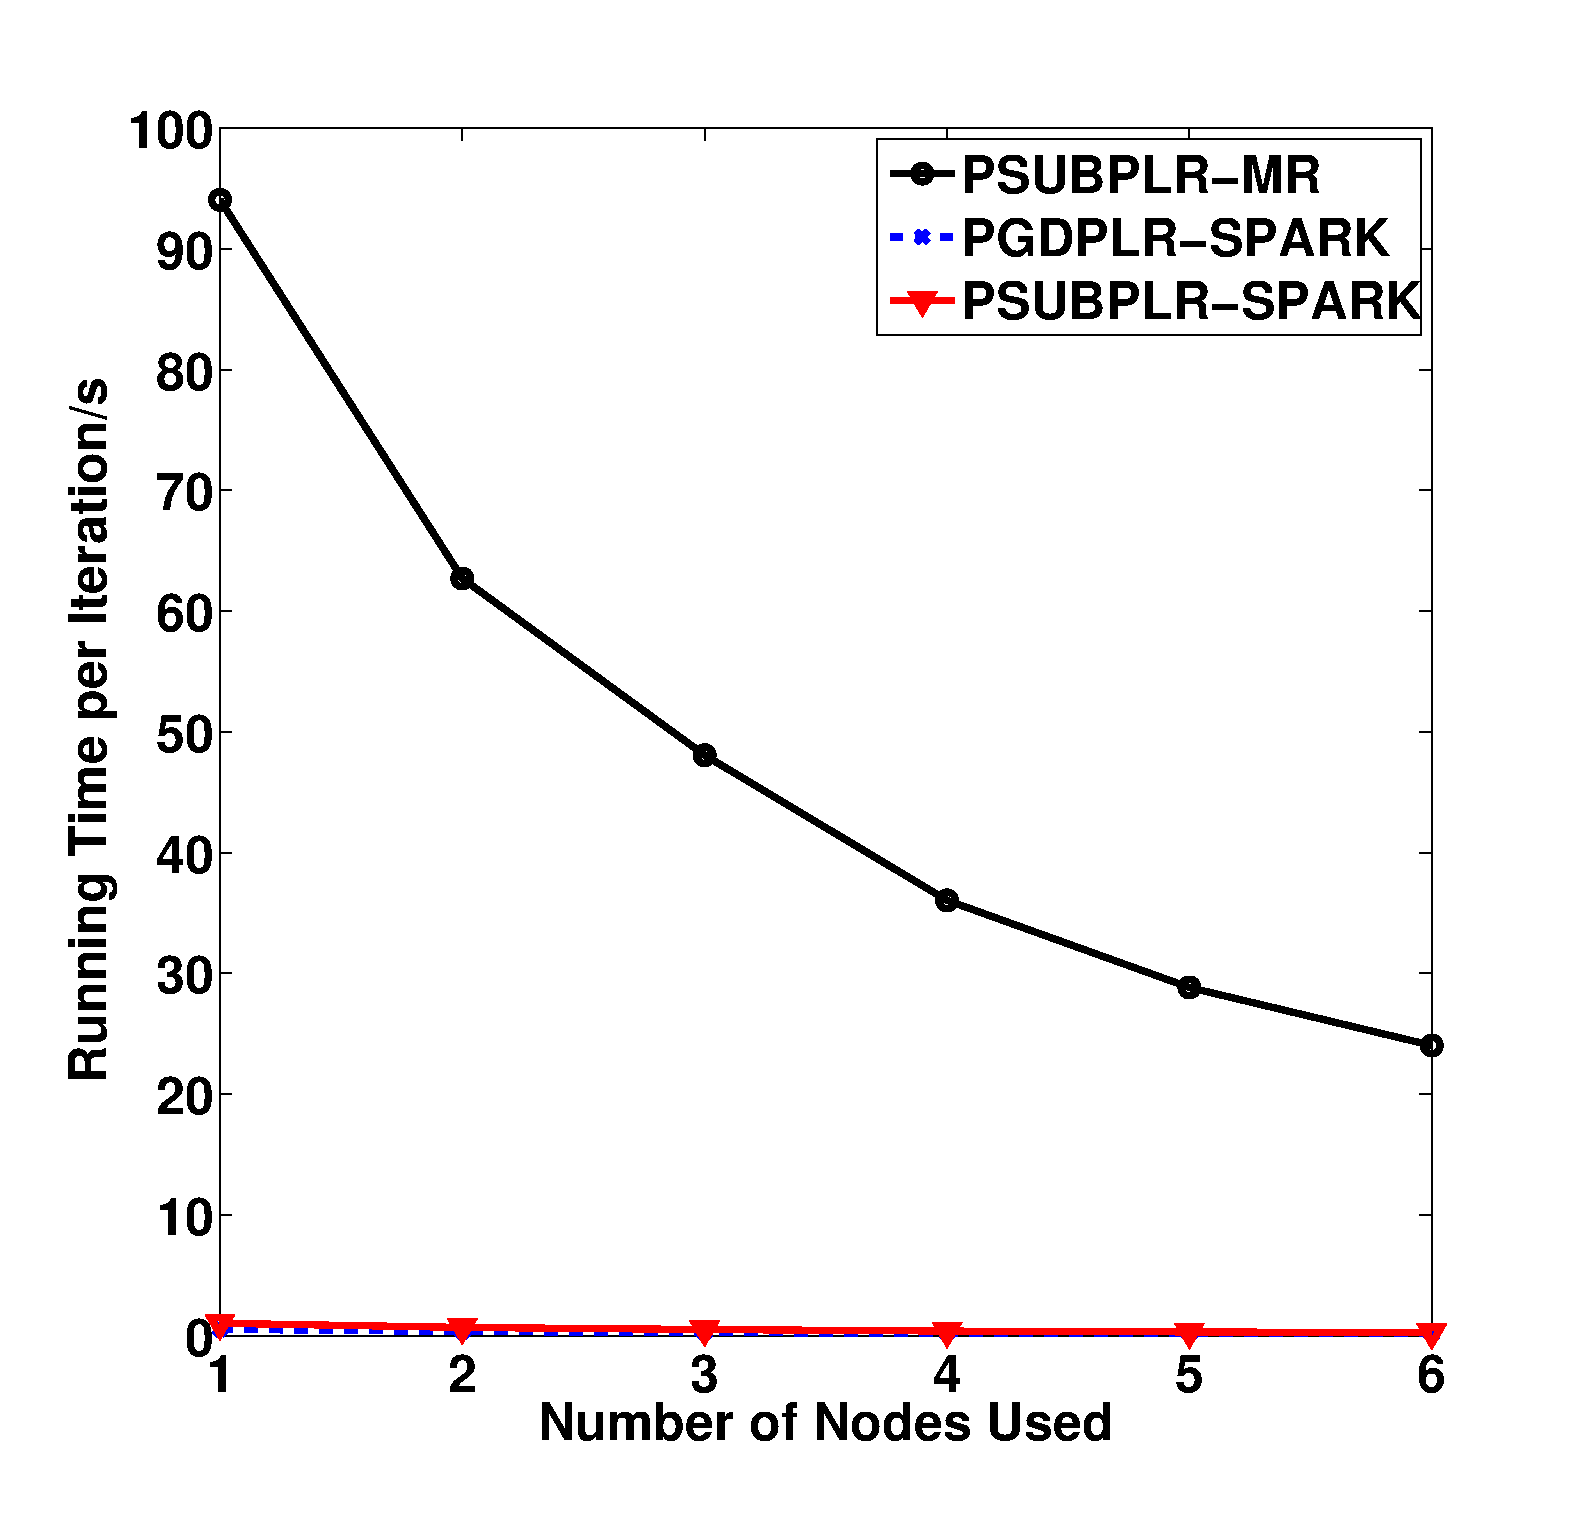
\includegraphics[height=4.5cm,width=5cm]{img/2d_time.eps}
\caption{Running time, as a function of used node number on Simulated \textbf{2d} Dataset}
\end{figure}

\begin{figure}[tb] \label{fig:10}
\center 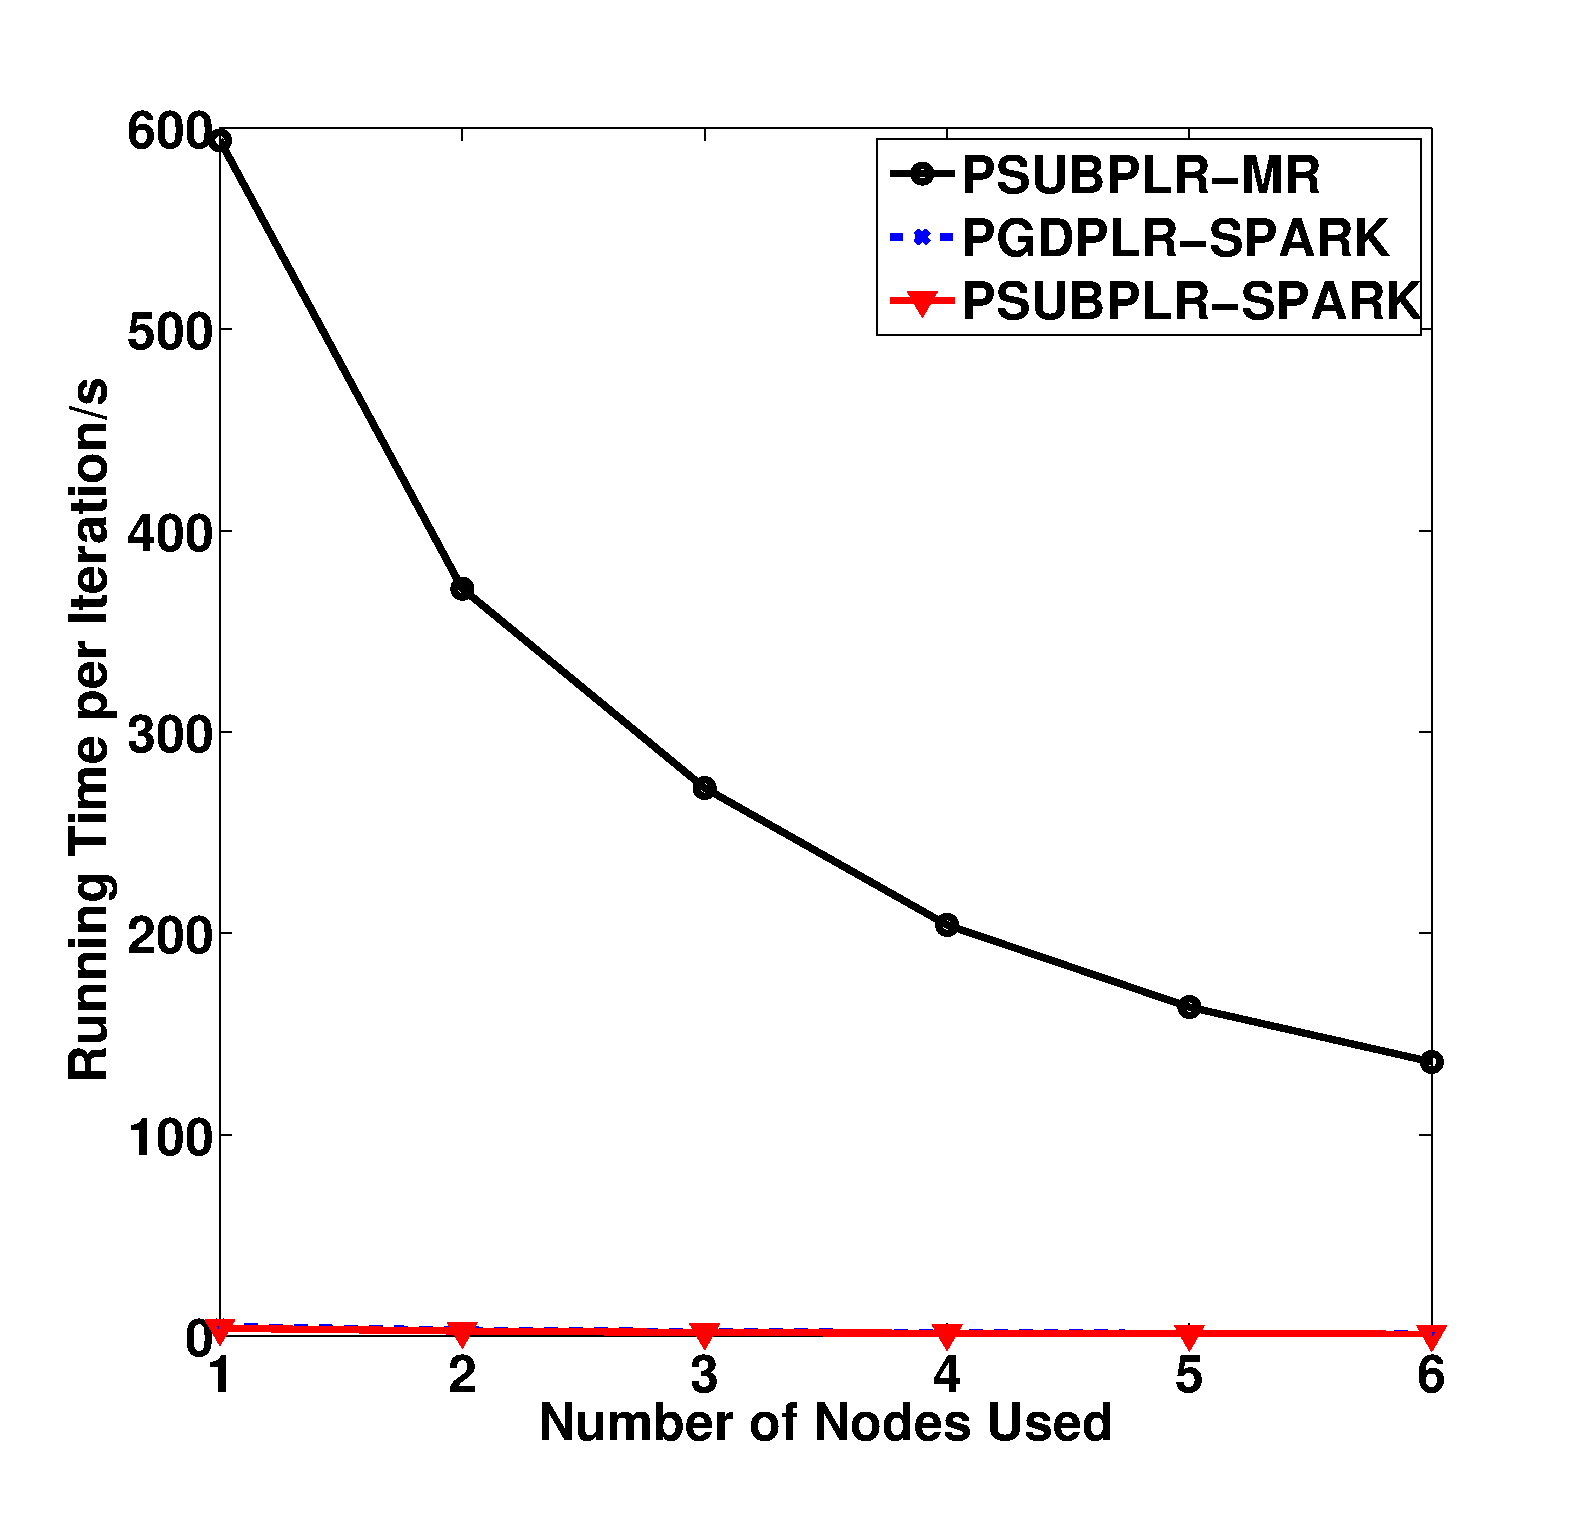
\includegraphics[height=4.5cm,width=5cm]{img/20NewsGroup_time.eps}
\caption{Running time, as a function of used node number on \textbf{20NewsGroup} Dataset}
\end{figure}

\begin{figure}[tb] \label{fig:11}
\center 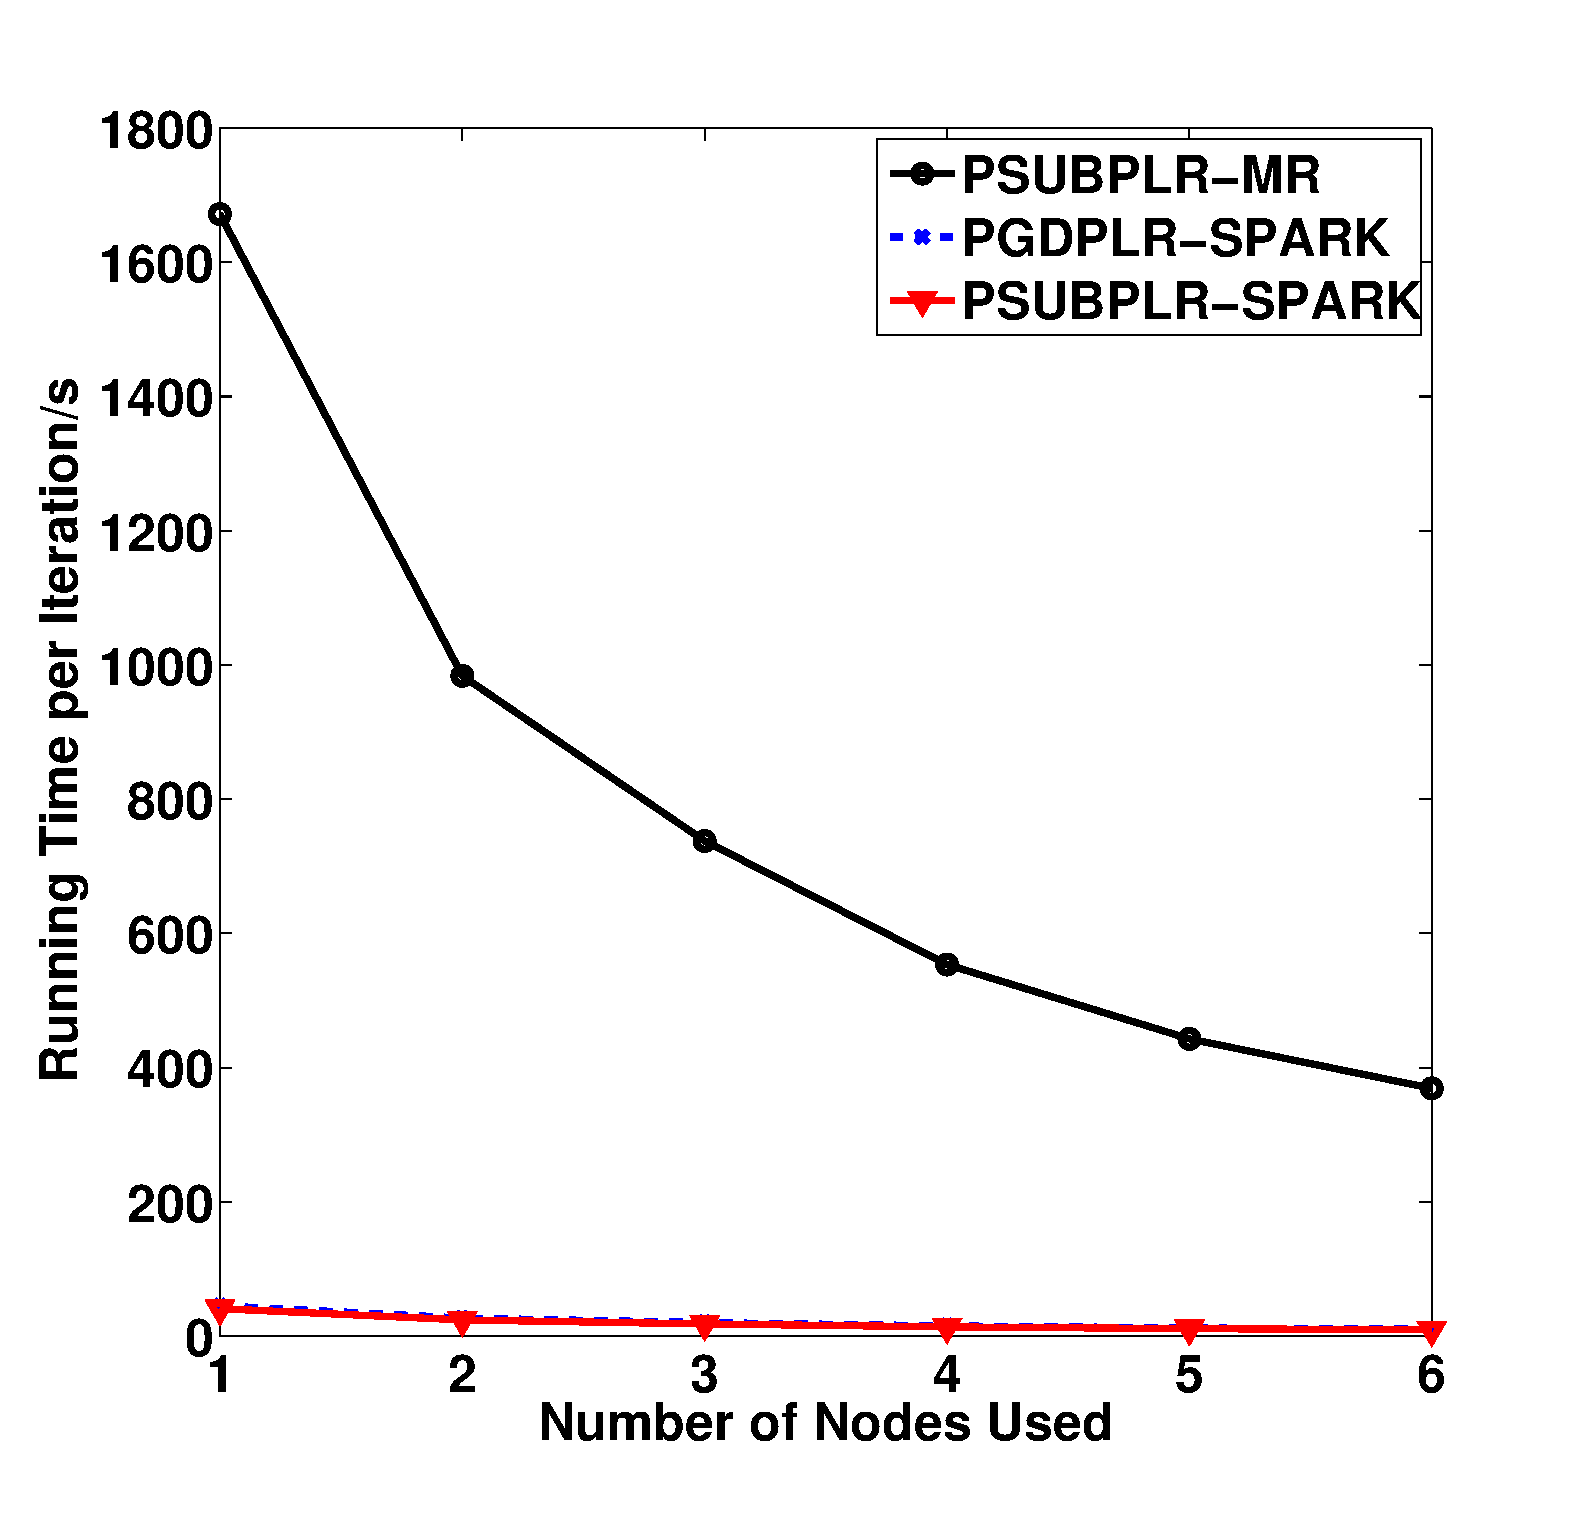
\includegraphics[height=4.5cm,width=5cm]{img/Gisette_time.eps}
\caption{Running time, as a function of used node number on \textbf{Gisette} Dataset}
\end{figure}

\begin{figure}[tb] \label{fig:12}
\center 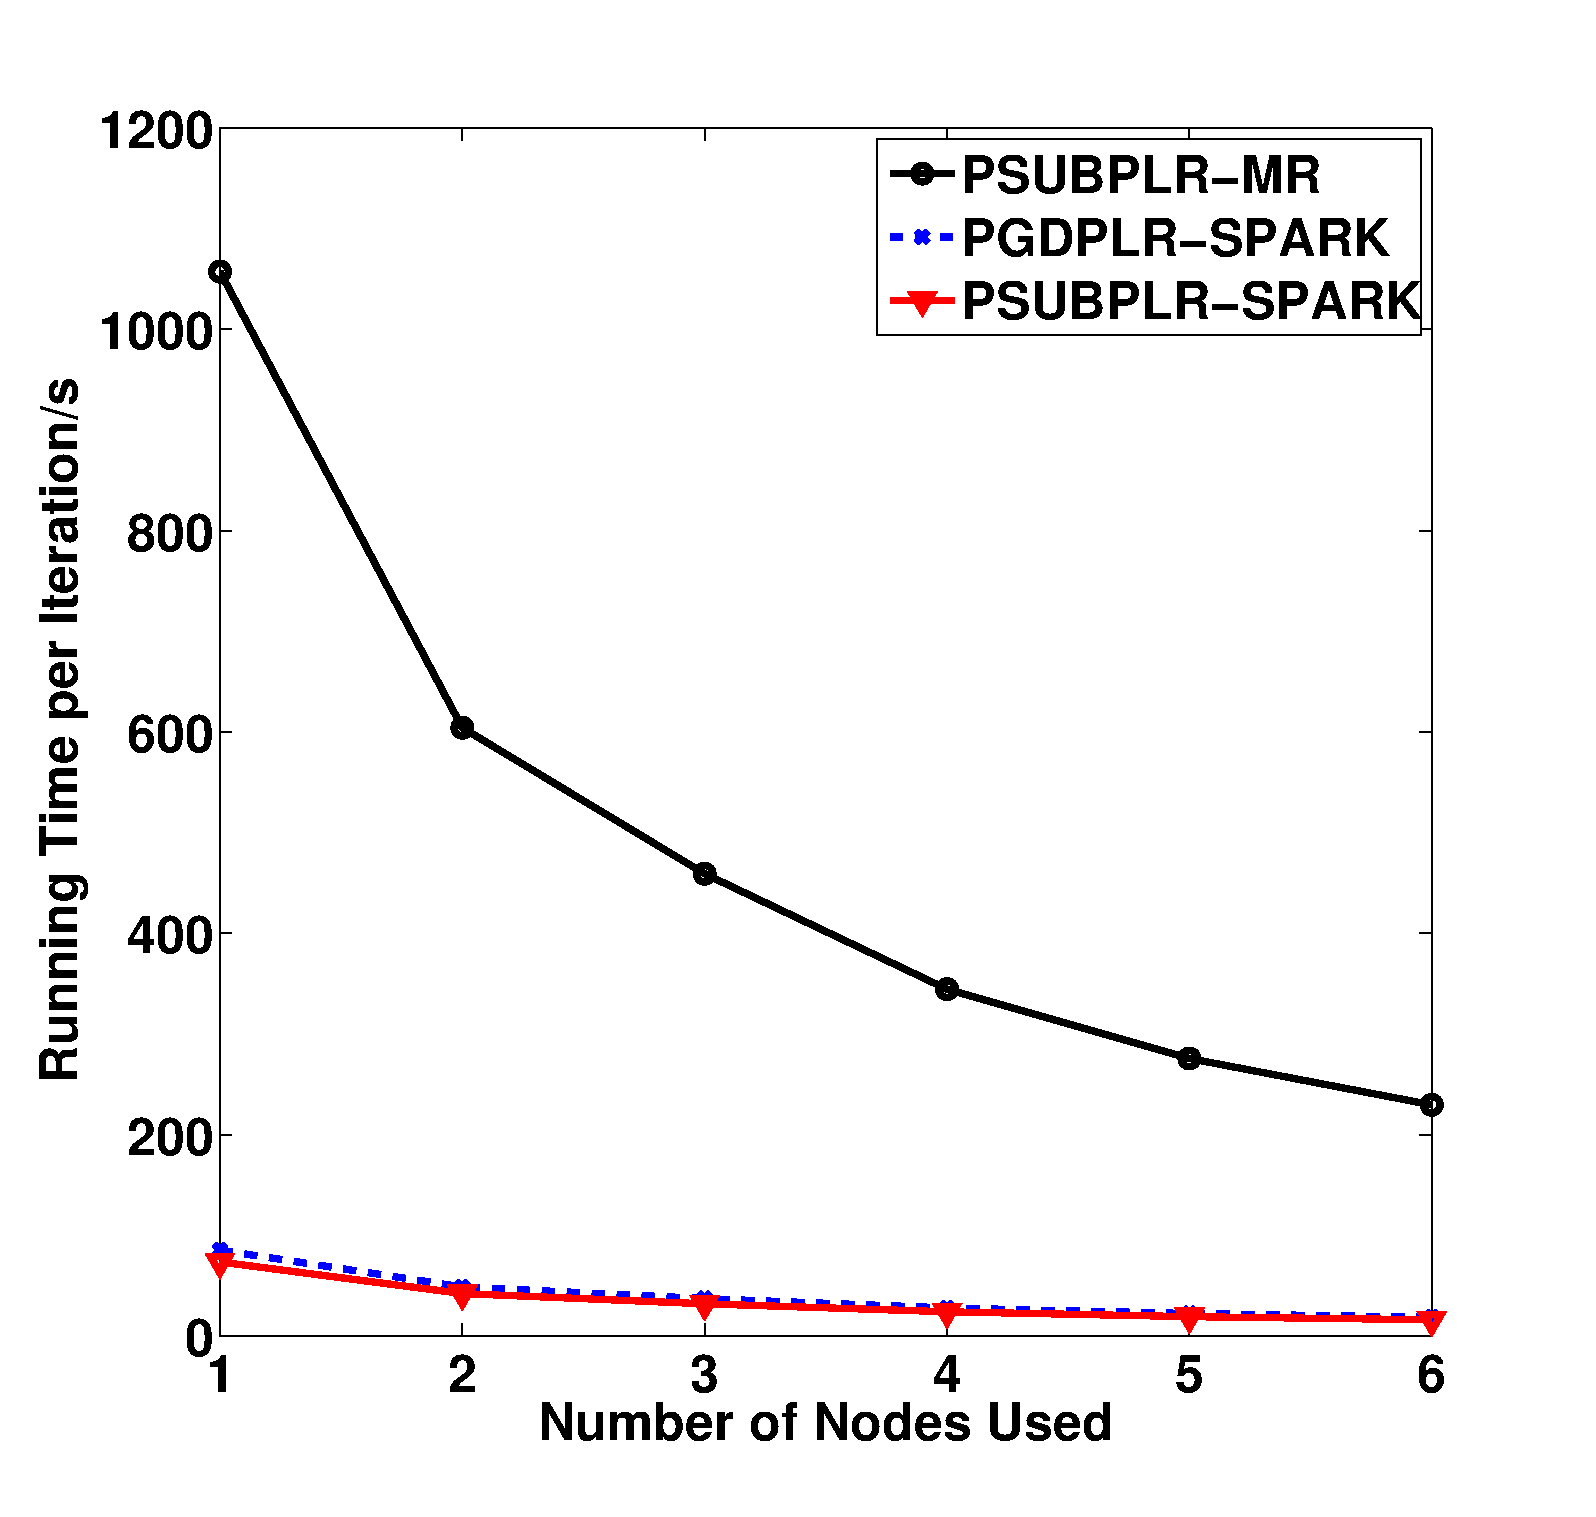
\includegraphics[height=4.5cm,width=5cm]{img/ECUESpam_time.eps}
\caption{Running time, as a function of used node number on \textbf{ECUESpam} Dataset}
\end{figure}

\begin{figure}[tb] \label{fig:13}
\center 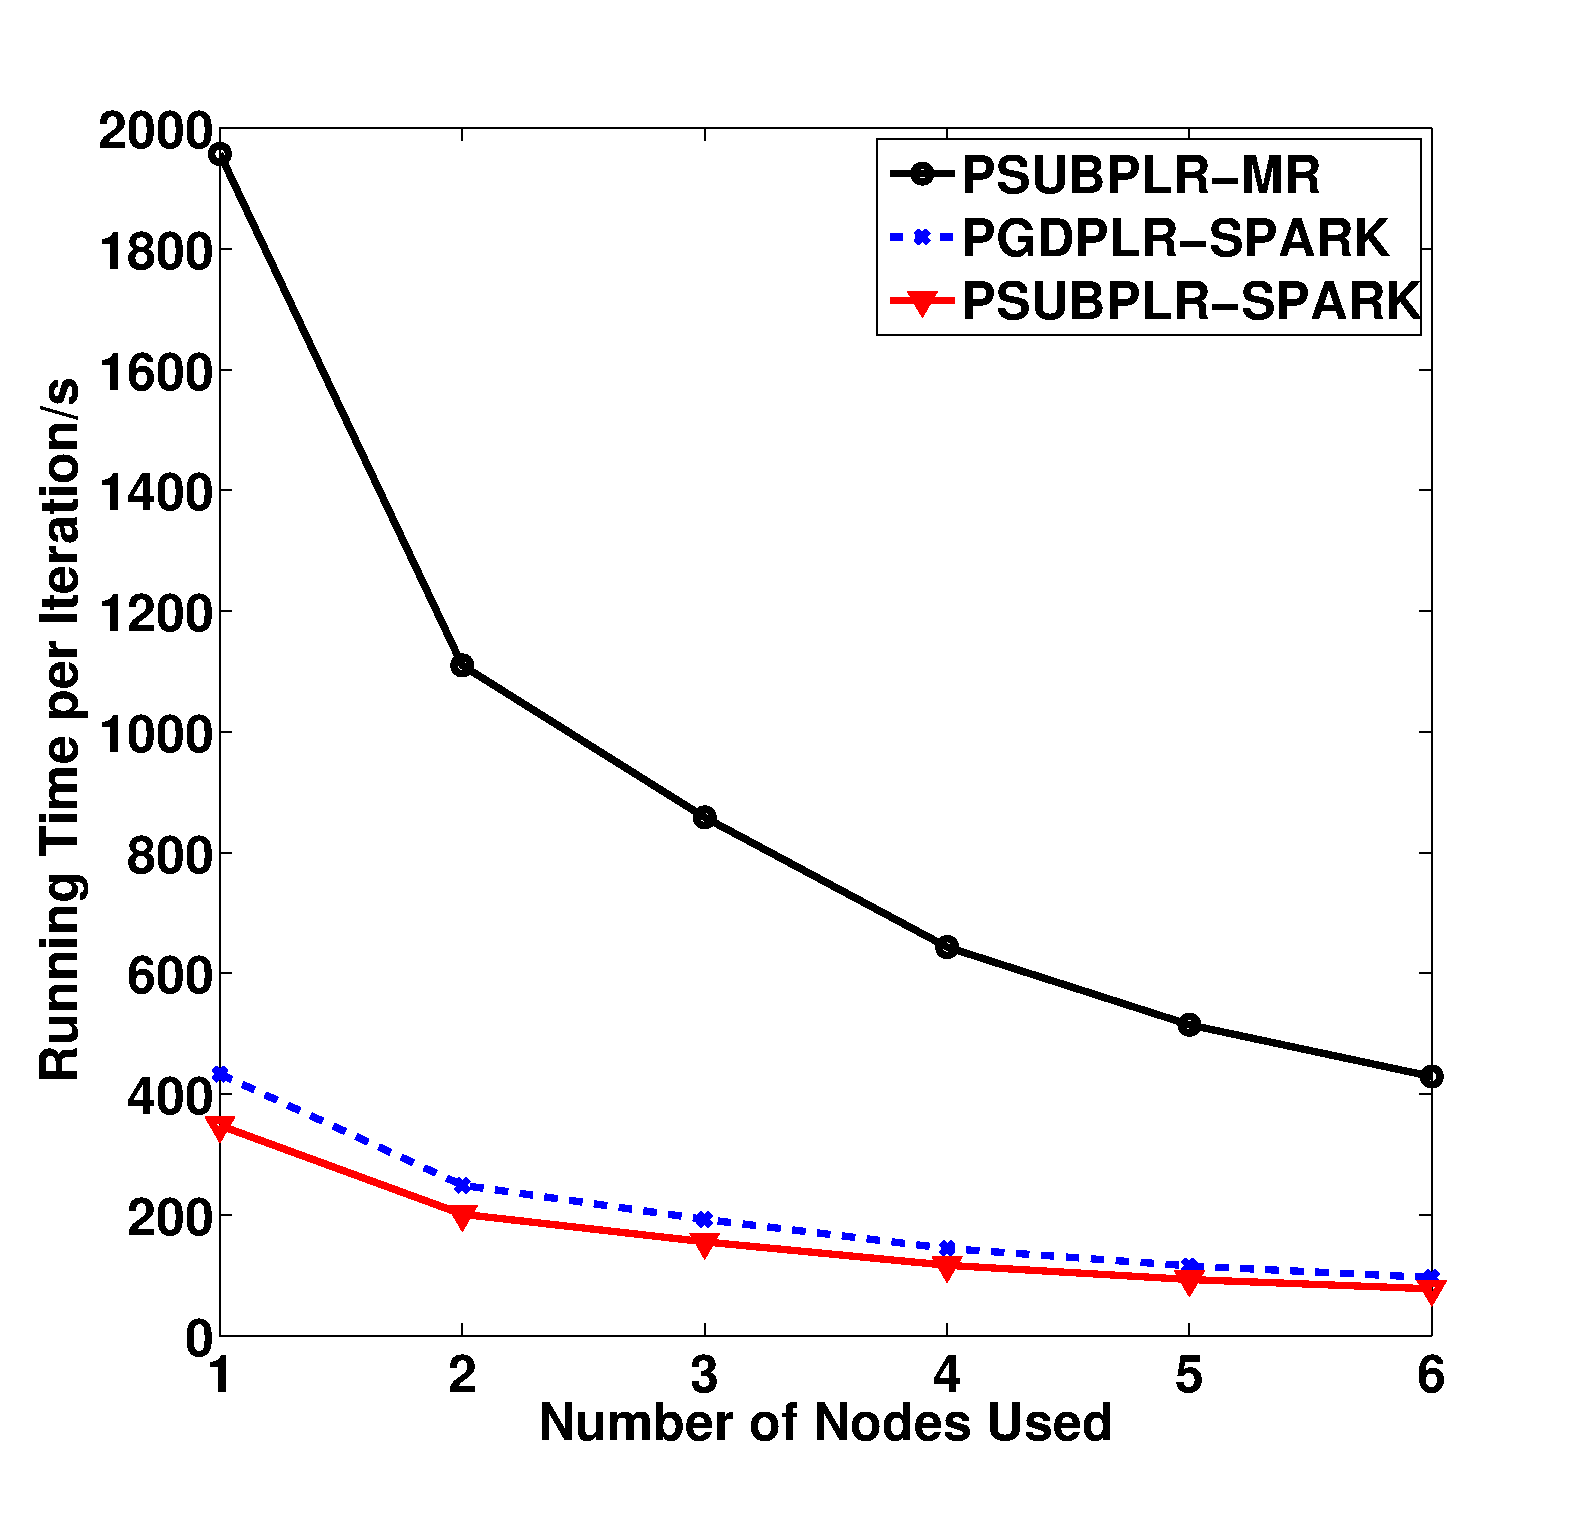
\includegraphics[height=4.5cm,width=5cm]{img/URL-Reputation_time.eps}
\caption{Running time, as a function of used node number on \textbf{URL-Reputation} Dataset}
\end{figure}

As we can see from the results, fewer computation resources provided, longer the implementation process will take.
However, this trend is not in a consistent fashion. When number of machines gets higher, the less impact it will make.
We may reach a point for every algorithm when running time stops decreasing as machine number increases.
This shows the true scalability of the designed algorithm, which we can study in our future work.

\subsection{Fault Tolerance}
There are both system level techniques and algorithm level techniques to provide fault tolerance in parallel computation.
Results are shown in Table~\ref{tab:table5}.
\begin{table}[h]
\centering
\caption{Fault Tolerance Analysis}\label{tab:table5}
\begin{tabular}{|c|c|c|}
\hline
           & System Level & Algorithm Level \\
\hline
Mahout     & \XSolid & \XSolid  \\
\hline
Liblinear  & \XSolid & \XSolid \\
\hline
SLLR  & \XSolid & \Checkmark \\
\hline
PSUBPLR-MR & \Checkmark & \Checkmark \\
\hline
PGDPLR-SPARK & \Checkmark & \XSolid \\
\hline
PSUBPLR-SPARK & \Checkmark &  \Checkmark \\
\hline
\end{tabular}
\end{table}
Here, randomization is employed in all sublinear methods, thus provides algorithm level fault tolerance for SLLR, PSUBPLR-MR and PSUBPLR-SPARK.
Hadoop and Spark can both provide fault tolerance, but in different ways. Hadoop employs HDFS while Spark has RDDs.
Of all six test programs, PSUBPLR-MR and PSUBPLR-SPARK are fault tolerant in both system level and algorithm level.

We show the iteration time as a function of percentage of failed maps on \textbf{URL-Reputation} dataset for all three parallel test programs in Fig.~\ref{fig:14}.
This is tested on 6 nodes.
\begin{figure}[tb] \label{fig:14}
\center 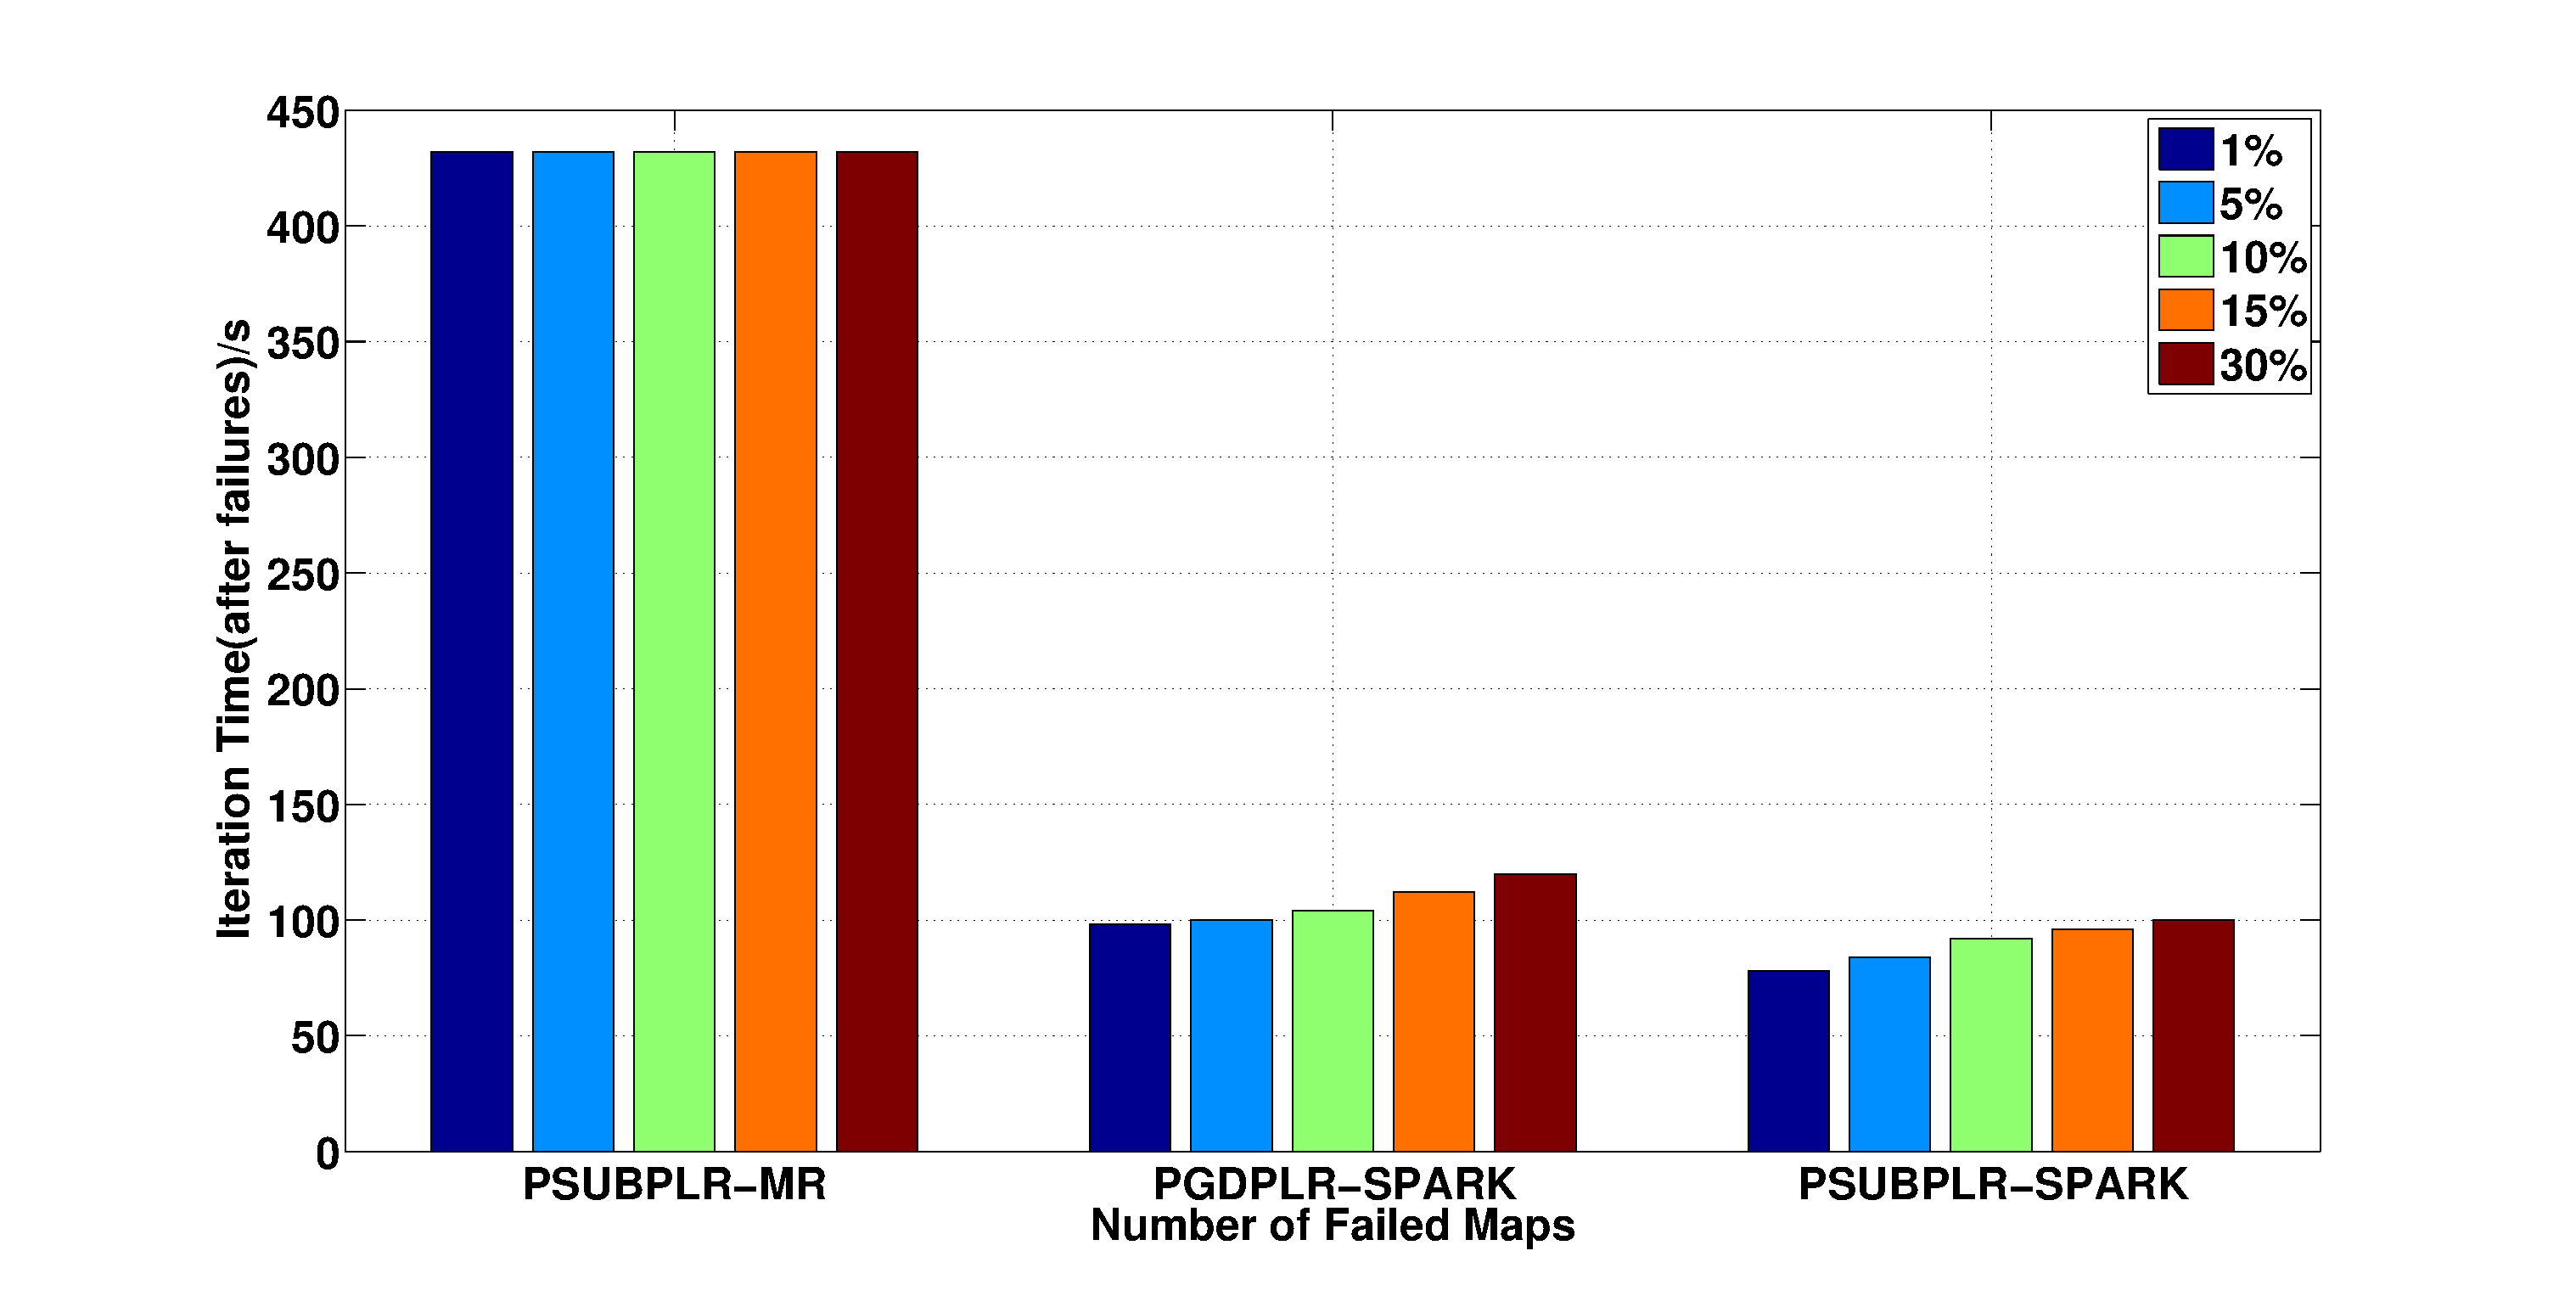
\includegraphics[height=4.5cm,width=9cm]{img/fault_tolerance.eps}
\caption{Iteration time, as a function of percentage of failed maps, on \textbf{URL-Reputation} Dataset, run on 6 nodes}
\end{figure}
As the outcome shows, PSUBPLR-MR suffers no running time increase per iteration when maps failed. But it takes the cost of precision loss if we enforce no additional iterations are implemented.
PGDPLR-SPARK and PSUBPLR-SPARK will increase iteration time right after the maps failed. It is due to RDD reconstruction. The increase is not significant.
This difference also proves the different mechanism of fault tolerance between Hadoop and Spark.

\section{Conclusion} \label{sec:concl}
In this paper we analyzed three optimization approaches along with three computing platforms to train LR model with large-volume, high-dimensional dataset for classification.
We focus on both algorithm design and choosing of computing platforms.
We tested correctness, learning accuracy, running time, scalability and fault tolerance of different programs.
These tests are objective, as the carefully chosen datasets range from KB to GB in size.
We also consider the sparsity issues in all real world datasets.
Test results show that different algorithms and different computing platforms have their own advantages.
We should choose wisely of the combination of algorithm and computing platform according to dataset situations and machine resources.
A minor contribution in this paper is to present a novel parallel sublinear algorithm for LR implemented on both Hadoop and Spark.
We realize this paper has its limitation in both machine resources and datasets.
It is exactly we are heading for: More machines and larger datasets will bring more convincing results.
We also plan to employ the research angle of combining algorithm design and computing platform to study other machine learning models, thus giving more valuable suggestions in practical applications.
 
\begin{small}
\bibliographystyle{plain}
\bibliography{mlpaper}
\end{small}
\end{document} 